\documentclass[10pt]{article}
\usepackage{NotesTeXV3,lipsum}
\usepackage{myMathHeader}
%\usepackage{showframe}

\begin{document}
    \title{{Notes for Differential Geometry}
        \\{\normalsize{\itshape Curves, Surfaces and Forms}}}
    \author{Tobias Diez}
    \affiliation{
        Shanghai Jiao Tong University\\
        \href{https://www.tobiasdiez.de}{Website}

        If you find any mistakes in these notes or have suggestions for improvements, please open an issue or a pull request on
        \href{https://github.com/tobiasdiez/LectureCurvesSurfaces/}{GitHub}.

        The initial version of these notes was written in 2024 by \emph{Jinghan Cai} as part of the lecture Differential Geometry of Curves and Surfaces at Shanghai Jiao Tong University.
    }
    \emailAdd{research@tobiasdiez.de}
    
    \maketitle

    \section*{Introduction}

    Curves and surfaces are fundamental objects in geometry and have been studied for thousands of years. 
    You have encountered them in various contexts, perhaps often without explicitly recognizing them as interesting mathematical entities: when you bind your shoes you entangle and bend curves; when you look at the shape of a leaf or a flower, you observe a beautiful surface in three-dimensional space; when you navigate using a map, you work with a flat representation of the curved surface of the Earth.
    
    The mathematical study of curves and surfaces is called differential geometry.
    Here, the term ``differential'' refers to the use of calculus, which allows us to analyze the local properties of these objects by examining how they change under infinitesimally small variations. One of the key challenges is then to understand how these local properties relate to the global structure of the objects.

    The aim of this course is to introduce you to the fundamental concepts and techniques of differential geometry, focusing on curves and surfaces in three-dimensional space.
    We will explore how to describe these objects mathematically and how to analyze their properties.

    The topics covered in this course have numerous applications in various fields, including physics, engineering, computer graphics, and more.
    To name a few examples:
    \begin{itemize}
        \item One of the most profound insights in modern physics is that the gravitational force can be understood as a manifestation of the curvature of space and time. This idea, introduced by Einstein's theory of general relativity, has revolutionized our understanding of the universe and has been confirmed by numerous experiments and observations. Similarly, the behavior of electromagnetic fields and the other elementary forces can be described using the geometry of curved objects.
        
        \item In engineering, the design of structures such as bridges and buildings often requires an understanding of the geometry to ensure stability and efficiency.
    
        \item The realistic rendering of three-dimensional objects in computer graphics relies on the mathematical description of surfaces and their properties, such as curvature and texture.
    \end{itemize}


    \newpage
    \part{Curves}\label{Part:Curves}

        \section{Parameterized curves}

            There are two ways to view a curve.
            Imagine you register for a mountain bike race.
            The race track, as marked by the organizers, exists independently of you and is described by a certain set of points in space.
            This one-dimensional object is what we call a \emph{curve}.
            However, as a participant in the race, you experience the curve differently: you move along it, and your position can be recorded at different times.
            This function, which maps time to your position in space, is what we refer to as a \emph{parameterized curve}.

            \begin{definition}[Curve]
                A \emphDef{parameterized curve} is a smooth map $c: I\to\R^n(n = 2, 3)$, where $I$ is an interval, usually $[a,b]$ or $(0,1)$.
                A \emphDef{curve} is the image of a parameterized curve, i.e., the set $\set{c(t) \given t\in I}$.
            \end{definition}

            Note that the parameter $t$ does not necessarily represent time; it can be any parameter that varies along the curve.
            For example, in the case of the bike race, $t$ could represent the distance traveled along the track instead of the time elapsed.
            Nonetheless, it is often convenient to think of $t$ as time, as it provides an intuitive way to understand the motion along the curve.
            In this spirit, we refer to $\dot{c}(t) = \difFrac{c}{t}$ as the velocity vector and $\ddot{c}(t) = \difFrac{\dot{c}}{t}$ as the acceleration vector.

            There are many different parameterizations for the same curve.
            For example, different riders may travel at different speeds, leading to different parameterizations of the same physical curve.
            So we need a way to pass from one parameterization to another.
            \begin{definition}[Diffeo\-morphism]
                A smooth map $\varphi: I_2\to I_1$ is called a \emphDef{diffeomorphism} if $\varphi$ is bijective (one-to-one and onto) and its inverse $\varphi^{-1}$ is also smooth.
            \end{definition}
            \begin{definition}[Repara\-meter\-iza\-tion]
                If $\varphi: I_2 \to I_1$ is a diffeomorphism with\footnote{A diffeomorphism $\varphi$ always has either $\varphi'(t) > 0$ or $\varphi'(t) < 0$ for all $t$. The latter case would correspond to reversing the direction of the curve.} $\varphi'(t) > 0$ and $c_1:I_1 \to \R^n$ is a parameterized curve, then $c_2(t) = c_1\bigl(\varphi(t)\bigr): I_2 \to \R^n$ is also a parameterized curve, called the \emphDef{reparameterization} of $c_1$ by $\varphi$.
            \end{definition}

            We will often introduce a certain property of the curve using a parameterization, and then show that this property does not depend on the choice of parameterization.
            For example, the length of a curve is a property that should be independent of how we parameterize it -- all riders should better agree on the length of the track, regardless of their speed.
            \begin{definition}[Length of a curve]
                The length of a parameterized curve $c: I \to \R^n$ is defined as
                \begin{equation}
                        L(c) \defeq \int_a^b \norm{\dot{c}(t)}\dif t
                \end{equation}
                where $I = [a,b]$ or $(a,b)$.
            \end{definition}

            \begin{lemma}
                If $c_2$ is a reparameterization of $c_1$, then the length of $c_1$ and $c_2$ are the same.
            \end{lemma}
            \begin{proof}
                Since $c_2(t) = c_1\bigl(\varphi(t)\bigr)$ for some diffeomorphism $\varphi: I_2\to I_1$, we have by the chain rule
                \begin{equation*}
                    \begin{aligned}
                        \difFracAt{}{t}{t} c_2 = \varphi'(t)\difFracAt{}{s}{\varphi(t)}c_1.
                    \end{aligned}
                \end{equation*}
                Assume, without loss of generality, that $I_1 = [a_1, b_1]$ and $I_2 = [a_2, b_2]$ with $\varphi(a_2) = a_1$ and $\varphi(b_2) = b_1$. Thus,
                \begin{equation*}
                    \begin{aligned}
                        L(c_2) &= \int_{a_2}^{b_2}\norm*{\difFracAt{}{t}{t} c_2}\dif t \\
                        &= \int_{a_2}^{b_2}\big|\varphi'(t)\big|\cdot\norm*{\difFracAt{}{s}{\varphi(t)}c_1}\dif t \\
                        &\stackrel{s=\varphi(t)}{=}\int_{a_1}^{b_1}\norm*{\difFracAt{}{s}{s} c_1}ds \\
                        &= L(c_1),
                    \end{aligned}
                \end{equation*}
                where we used the reparameterization theorem for integrals in the third step.
                \footnotetext{The proof exhibits a general strategy that we will use often in this course: when we want to investigate a certain property of a curve or surface, we will use a parameterization to boil it down to a problem in calculus that we know how to solve. Here, we just used the chain rule and the reparameterization theorem for integrals.}
            \end{proof}
            
            At this point, a word of caution is in order.
            In the definition of a curve, we required the parameterization to be smooth (i.e, all derivatives exist and are continuous).
            However, this does not imply that the curve itself is smooth in a geometric sense.
            For example, the parameterization $c(t) = (t^3, t^2)$ is smooth, but the curve it describes has a cusp at the origin.
            \begin{figure}[H]
                \centering
                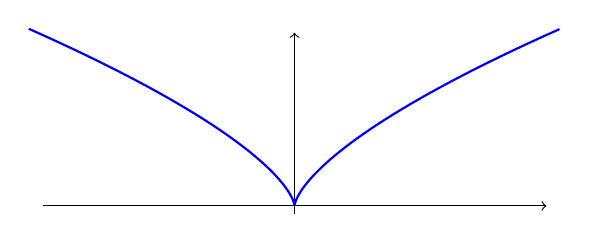
\begin{tikzpicture}
                    \draw[->] (-3.2,0) -- (3.2,0);
                    \draw[->] (0,-0.1) -- (0,2.2);

                    \draw[thick, blue, samples=100, domain=-1.5:1.5] plot (\x*\x*\x, \x*\x);
                \end{tikzpicture}
                \caption{Plot of the smooth curve $c(t) = (t^3, t^2)$ showing a cusp at the origin.}
            \end{figure}
            To avoid such singularities, we introduce the following definition.

            \begin{definition}[Regular curve]
                A parameterized curve $c$ is called \emphDef{regular} if $\dot{c}(t)\neq 0$ for all $t\in I$.
                Such a curve, in particular, has no cusps or corners.
            \end{definition}
    
            The regularity condition ensures that the curve has a well-defined, non-zero tangent vector at every point, which is crucial for many applications in differential geometry.
            We will almost always assume that the curves we work with are regular.
            The following result shows that every regular curve can be reparameterized to have unit speed, which is often a convenient choice.
            \begin{proposition}
                For every regular curve $c: I \to \R^n$, there exists a diffeomorphism $\varphi: I \to I$ such that $\Tilde{c}(s) = c\big(\varphi(s)\big)$ has unit-speed, i.e., $\norm{\dot{\Tilde{c}}(s)} = 1$ for all $s\in I$.
            \end{proposition}
            A curve $c(t)$ with unit-speed is also called an \emphDef{arc-length parameterization} of the curve, since the parameter $t$ directly measures the length along the curve from some starting point.
            Indeed, if we let $l(t) = \int_{t_0}^{t} \norm{\dot{c}(\tau)} \dif \tau$ be the length of the arc from a given point $c(t_0)$ to $c(t)$, then for a unit-speed curve, we have $l(t) = t - t_0$.

            For a unit-speed curve, the velocity vector $\dot{c}(t)$ has unit length by definition.
            We can use the acceleration to find a second vector $N(t)$ that is perpendicular to $\dot{c}(t)$ and also has unit length.
            \begin{theorem}[Moving frame]
                Let $c: I\to\R^n$ be a unit-speed curve with $\ddot{c}(t)\neq 0$ for all $t$, then 
                \begin{equation}
                    T(t) \defeq \dot{c}(t), \quad N(t) \defeq \cfrac{\ddot{c}(t)}{\norm{\ddot{c}(t)}}                
                \end{equation}
                have unit length and are perpendicular to each other, i.e., they form a pair of orthonormal vectors.
            \end{theorem}
            If the curve lies in $\R^2$, then we get two orthonormal vectors $T(t)$ and $N(t)$ that span $\R^2$, i.e., an orthonormal basis of $\R^2$ that moves along the curve.
            This is called a \emphDef{moving or Frenet--Serret frame} along the curve.

            \begin{definition}[Curvature]
                The curvature of a unit-speed curve $c: I\to\R^n$ is defined as $\kappa(t) = \norm{\ddot{c}(t)}$.
            \end{definition}
            What is the curvature of a general regular curve $c: I\to\R^n$?
            The natural definition is to first reparameterize $c$ to a unit-speed curve $\Tilde{c}$ by a suitable reparameterization $\varphi$ and then define the curvature of $c$ as the curvature of $\Tilde{c}$.
            One has to be a bit careful here to measure the curvature at the same point on the curve:
            If $c(t)$ is a point on the curve, then $\Tilde{c}(s) = c\big(\varphi(s)\big)$ is the same point if $s = \varphi^{-1}(t)$.
            Accordingly, we define the curvature $\kappa(t)$ of $c$ at $t\in I$ as the curvature $\tilde{\kappa}(s)$ of $\Tilde{c}$ at $s = \varphi^{-1}(t)$, i.e., 
            \begin{equation}
                \kappa(t) = \tilde{\kappa}\bigl(\varphi^{-1}(t)\bigr).
            \end{equation}
            \begin{lemma}
                If $c: I\to\R^n$ is a regular curve, then its curvature is given by
                \begin{equation}
                    \kappa(t) = \frac{1}{v(t)^2}\sqrt{\norm{\ddot{c}(t)}^2 - \dot{v}(t)^2} = \frac{\sqrt{v(t)^2\norm{\ddot{c}(t)}^2 - \bigl(\dot{c}(t) \cdot \ddot{c}(t)\bigr)^2}}{v(t)^3},
                \end{equation}
                where $v(t) = \norm{\dot{c}(t)}$ is the speed of $c$ at time $t$.
            \end{lemma}
            \begin{proof}
                Homework.
            \end{proof}

            The 1-order approximation of a curve is tangent line, while the 2-order approximation is osculating circle.

        \section{Moon in the puddle}

            One of the overarching themes in differential geometry is to understand how local properties of a curve or surface relate to its global structure.
            The theorem about the Moon in a puddle is a beautiful example of this idea.
            It answers the question: If a curve is not too tightly curved, what can we say about the region it encloses?


            To understand the theorem, we first need to introduce a few concepts.
            \begin{definition}[Loop]
                A parameterized curve $c: [a,b] \to \R^n$ is called a \emphDef{loop} if $c(a) = c(b)$ and all (one-sided) derivatives of $c$ agree at $a$ and $b$, i.e., $\difFracAt{^k}{t^k}{t=a} c(t) = \difFracAt{^k}{t^k}{t=b} c(t)$ for all $k\ge 1$.
                It is called \emphDef{simple} if it does not intersect itself, i.e., $c(t_1)\neq c(t_2)$ for all $t_1, t_2\in [a,b)$ with $t_1\neq t_2$.
            \end{definition}
            \begin{theorem}[Jordan curve theorem]
                Every simple loop in $\R^2$ divides $\R^2$ into two sets: one is bounded, called the inside; one is unbounded, called the outside.
            \end{theorem}

            A classical result about simple curves is the isoperimetric inequality, which states that among all simple loops with a given length, the circle encloses the largest area.
            \begin{theorem}[Isoperimetric inequality]
                Let $c: [a,b]\to\R^2$ be a simple loop in $\R^2$ of length $L$ enclosing an area $A$, then
                \begin{equation*}
                    4\pi A \le L^2,
                \end{equation*}
                with equality if and only if $c$ is a circle.
            \end{theorem}

            The isoperimetric inequality is a statement about the relationship between two global properties: the length of a curve and the area it encloses.
            In contrast, the theorem about the Moon in a puddle is a local-to-global result that connects the local property of curvature to the global property of enclosing a unit disc.
            The following lemma is the key step in the proof of the theorem.
            \begin{lemma}
                Suppose we have a simple, regular loop $c:I\to\R^2$. Then there exists a time $t_0\in I$ such that the osculating circle at $c(t_0)$ exists and lies inside of $c$.
            \end{lemma}
            \begin{figure}[H]
                \centering
                \includegraphics[width = 1\textwidth]{pic/Moon in the puddle.png}
                \caption{Note that maximal circle $C_p$ at $p$ has to touch loop $c$ at another point $q$, but for $C_{p_{\infty}}$, $q_{\infty} = p_{\infty}$ -- a contradiction.}
            \end{figure}
            \begin{theorem}[``Moon in the puddle'']
                Let $c: I\to\R^2$ be a simple, regular loop. If $\kappa(t)\le 1$ for all $t\in I$, then the region surrounded by $c$ contains a unit disc.
            \end{theorem}
            \begin{proof}
                By the lemma, there exists a point $p = c(t_0)$ on the curve such that the osculating circle $\sigma$ at $p$ lies inside of $c$.
                But $\sigma$ has radius $r = \sfrac{1}{\kappa(t_0)} \ge 1$, so it contains a unit disc.
            \end{proof}

        \section{Winding number}
            Another common theme in differential geometry is that the integral of a local quantity over a closed curve or surface often yields a discrete global invariant of the object.

            For example, consider a simple loop $c: [a, b] \to \R^2$ in the plane that does not pass through the origin.
            Then we can look at the expression 
            \begin{equation}
                \frac{1}{2\pi}\int_a^b \frac{x(t)\dot{y}(t) - y(t)\dot{x}(t)}{x(t)^2 + y(t)^2} \dif t.
            \end{equation}
            A priori, this integral could take any real value.
            And you might expect that if you deform the curve slightly, the integrand would change continuously, and thus the value of the integral would also change continuously.
            However, this is not the case.
            The integral actually takes on only integer values and remains invariant under continuous deformations of the curve that do not pass through the origin.

            To understand why this is true, it is helpful to start from the following geometric notion.

            \begin{definition}[Winding number]
                Let $c: [a, b]\to\R^2$ be a loop and $P_0$ be a point that does not lie on the curve.
                The winding number $W(c, P_0)$ is the number of times the curve goes counter-clockwise around $P_0$.
            \end{definition}

            From geometric considerations, it is clear that the winding number is an integer that satisfies the following properties:
            \begin{proposition}
                \begin{itemize}
                    \item $W(c, P_0)$ depends on $P_0$;
                    \item $W(c, P_1) = W(c, P_2)$ if $P_1$ and $P_2$ can be connected by a curve not intersecting $c$.
                    \item $W(c, P_0)$ is invariant under continuous deformations of $c$ that do not pass through $P_0$, i.e., if $c_\delta$ is a family of loops with $c_\delta(t)\neq P_0$ for all $\delta, t$, then $W(c_\delta, P_0)$ is independent of $\delta$.
                \end{itemize}
            \end{proposition}

            To get a formula for the winding number, we first shift the curve so that $P_0$ is at the origin.
            Then we can express the curve in polar coordinates\footnote{Strictly speaking, we view $\theta$ here as a smooth real-valued function of $t$ (and not modulo $2\pi$). This is possible because the polar coordinates furnish a covering map $(r, \theta) \mapsto r \Vector{\cos\theta, \sin\theta}$ from $(0, \infty) \times \R$ to $\R^2 \setminus \set{0}$. Then, using the lifting property of covering spaces, we can lift the curve $c$ in $\R^2 \setminus \set{0}$ to a curve in $(0, \infty) \times \R$, whose coordinates are exactly the functions $r(t)$ and $\theta(t)$.} $c(t) = r(t) (\cos\theta(t), \sin\theta(t))$ with $r(t) > 0$ for all $t$.
            Since the curve is a loop, we have $r(a) = r(b)$ and $\theta(b) = \theta(a) + 2k\pi$ for some integer $k$.
            Clearly $k$ is the winding number of $c$ around the origin.
            To find a formula for $k = \frac{\theta(b) - \theta(a)}{2\pi}$, we will find an expression for $\dot{\theta}(t)$ and then integrate it over $[a,b]$.
            Denoting the components of $c(t)$ by $x(t)$ and $y(t)$, we have
            \begin{equation}\begin{split}
                \Vector{\dot{x} \\ \dot{y}}
                    = \dot{c}
                    &= \dot{r} \Vector{\cos\theta \\ \sin\theta} + r\dot{\theta} \Vector{-\sin\theta \\ \cos\theta} \\
                    &= \frac{\dot{r}}{r} \Vector{x \\ y} + \dot{\theta} \Vector{-y \\ x}.
            \end{split}\end{equation}
            Taking the dot product of both sides with $(-y, x)$, we conclude that
            \begin{equation}
                \dot{\theta} = \frac{x\dot{y} - y\dot{x}}{x^2 + y^2}.
            \end{equation}
            To find the winding number, we can integrate $\dot{\theta}$:
            \begin{equation}
                W(c, 0) = \frac{\theta(b) - \theta(a)}{2\pi} = \frac{1}{2\pi} \int_a^b \frac{x\dot{y} - y\dot{x}}{x^2 + y^2} \dif t.
            \end{equation}
            This is exactly the integral we started with!

        \section{Frenet-Serret frames for curves in $\R^3$}
            Curves in $\R^3$ can
            \begin{itemize}
                \item bend: measured by curvature (how much the curve deviates from being a straight line in a plane)
                \item twist: measured by torsion (how much this plane rotates along the curve)
            \end{itemize}

            \begin{definition}[Frenet-Serret frame]
                Let $c$ be a unit-speed curve in $\R^3$, $T(t) = \dot{c}(t)$ be the tangent field, curvature $\kappa(t) = |\ddot{c}(t)|$. Assume $\kappa(t)>0$, then $N(t) = \cfrac{\ddot{c}(t)}{|\ddot{c}(t)|}$, and $B(t) = T(t)\times N(t)$ is the binormal field. Here $\set{T,N,B}$ is called the Frenet-Serret frame.
            \end{definition}
            \begin{remark}
                $T(t), N(t), B(t)$ are orthogonal to each other and have unit length; notice that $|v\times w| = (v,v)(w,w) - (v,w)^2$.
            \end{remark}
            \begin{theorem}[Frenet-Serret equations]
                If $c: I\to\R^3$ is a unit-speed curve with F-N frame $T, N, B$, then
                \begin{equation}
                    \difFrac{}{t} \Vector{T \\ N \\ B} =
                    \Matrix{
                            0 & \kappa & 0 \\
                            -\kappa & 0 & \tau \\
                            0 & -\tau & 0 \\
                    }
                    \Vector{T \\ N \\ B}
                \end{equation}
                where $\tau(t) = -\dot{B}(t)\cdot N(t) = \dot{N}(t) \cdot B(t)$ is called the torsion of $c$ at $t$.
            \end{theorem}

            \begin{remark}
                The matrix
                \begin{equation}
                    \Omega = \Matrix{
                            0 & \kappa & 0 \\
                            -\kappa & 0 & \tau \\
                            0 & -\tau & 0 \\
                    }
                \end{equation}
                tells us how the Frenet-Serret frame changes along the curve.
                So if $T, N, B$ are the frame vectors at time $t$, then at time $t + \Delta t$, the frame vectors are approximately
                \begin{equation}
                    (1 + \Delta t \, \Omega) \Vector{T \\ N \\ B}.
                \end{equation}
                The fact that $\Omega$ is skew-symmetric (i.e., $\Omega^T = -\Omega$) means that the transformation $1 + \Delta t \, \Omega$ is an infinitesimal rotation.
                Geometrically, this means that as we move along the curve, the Frenet-Serret frame rotates in a way that is determined by the curvature and torsion of the curve.

                To extract the axis of rotation, note that the Frenet-Serret equations can be written also in the form
                \begin{equation}
                    \difFrac{}{t} \Vector{T \\ N \\ B} = \big(\tau T+\kappa B\big) \times \Vector{T \\ N \\ B}.
                \end{equation}
                In other words, the frame rotates about the axis given by the vector $\tau T + \kappa B$.
                This shows that the curvature measures the rotation about the binormal axis $B$, while the torsion measures the rotation about the tangent axis $T$.
                For this reason, the vector $\tau T+\kappa B$ is referred to as the instantaneous angular velocity vector of the curve (it is also called the Darboux vector).
            \end{remark}

            To explore the geometric meaning of curvature and torsion, we can use the Frenet-Serret frame as a local coordinate system and then study the behavior of the curve in these coordinates.
            For this purpose, let $c: I\to\R^3$ be a unit-speed curve with $\kappa(t) > 0$ for all $t\in I$, and let $T(t), N(t), B(t)$ be the Frenet-Serret frame.
            We can Taylor-expand $c(t)$ around a fixed time, which we take for simplicity to be $t = 0$:
            \begin{equation*}
                \begin{aligned}
                    c(t) \approx c(0) + t\thinspace\dot{c}(0) + \cfrac{t^2}{2}\thinspace\ddot{c}(0) + \cfrac{t^3}{6}\dddot{c}(0) + \cdots
                \end{aligned}
            \end{equation*}
            Using the Frenet-Serret equations, we can express the derivatives of $c$ in terms of $\kappa$ and $\tau$ as follows:
            \begin{equation*}
                \begin{aligned}
                    &\dot{c}(0) = T(0), \\
                    &\ddot{c}(0) = \kappa(0)\cdot N(0), \\
                    &\dddot{c}(0) = \difFracAt{}{t}{t=0} (\kappa N) = \dot{\kappa}(0)N(0) + \kappa(0)\bigg( -\kappa(0)T(0) + \tau(0)B(0) \bigg).
                \end{aligned}
            \end{equation*}
            Thus,
            \begin{equation*}
                \begin{aligned}
                    c(t) &\approx c(0) + \bigg( t - \kappa(0)^2\cfrac{t^3}{6} \bigg)T(0) + \bigg( \kappa(0)\cfrac{t^2}{2} + \dot{\kappa}(0)\cfrac{t^3}{6}\bigg)N(0) + \bigg( \kappa(0)\tau(0)\cfrac{t^3}{6} \bigg)B(0) \\
                    &\approx c(0) + T(0)t + \kappa(0)N(0)\cfrac{t^2}{2} + \kappa(0)\tau(0)B(0)\cfrac{t^3}{6},
                \end{aligned}
            \end{equation*}
            where in the last step we dropped the higher-order terms in $t$ for each component.
            This shows that:
            \begin{itemize}
                \item To first order, the curve looks like a straight line in the direction of $T$.
                \item To second order, the curve is a parabola in the plane spanned by $T$ and $N$, and the curvature $\kappa$ determines how tightly the curve bends in this plane.
                \item To third order, the curve starts to twist out of the plane spanned by $T$ and $N$, and the torsion $\tau$ measures the rate of this twisting.
            \end{itemize}
            From this geometric interpretation, the following proposition is quite intuitive.
            \begin{proposition}
                Let $c: I\to\R^3$ be a unit-speed curve with $\kappa > 0$.
                Then $c$ lies in a plane if and only if $\tau = 0$.
            \end{proposition}
            \begin{proof}
                $\Longrightarrow$: If $c$ lies in a plane, that plane has to be spanned by $T$ and $N$ which implies that $B$ is pointing in a fixed direction. 
                From the Frenet-Serret equations, it now follows that $\tau = 0$.
            
                $\Longleftarrow$: If $\tau = 0$, then $\dot{B}(t) = 0$, so $B(t) = B(0)\in\R^3$.
                Claim: $c$ lies in the plane orthogonal to $B$.
                To confirm the claim, we have to show that the following function is identically zero:
                \begin{equation*}
                    f(t) = \bigg( c(t) - c(0) \bigg)\cdot B(0).
                \end{equation*}
                But, since $\dot{c}(t) = T(t)$ is orthogonal to $B(t) = B(0)$, we have
                \begin{equation*}
                    \dot{f}(t) = \dot{c}(t)\cdot B(0) = 0.
                \end{equation*}
                Thus, $f(t)$ is constant and we conclude that $f(t) = f(0) = 0$.
            \end{proof}

            We saw that the curvature and torsion of a curve determine the local behavior of the curve up to third order.
            A natural question is whether they also determine the curve globally.
            Suppose we have two unit-speed curves $c, \Bar{c}$ with the same curvature $\kappa$ and torsion $\tau$.
            In order to compare their Frenet-Serret frames, we introduce the following function:
            \begin{equation*}
                f(t) = \cfrac{1}{2}\thinspace\big|T-\Bar{T}\big|^2 + \cfrac{1}{2}\thinspace\big|N-\Bar{N}\big|^2 + \cfrac{1}{2}\thinspace\big|B-\Bar{B}\big|^2
            \end{equation*}
            Then, we compute the derivative:
            \begin{equation*}
                \dot{f}(t) = \big(\dot{T} - \dot{\Bar{T}}\big)\big(T-\Bar{T}\big) + \big(\dot{N} - \dot{\Bar{N}}\big)\big(N-\Bar{N}\big) + \big(\dot{B} - \dot{\Bar{B}}\big)\big(B-\Bar{B}\big) = 0
            \end{equation*}
            where we used the Frenet-Serret equations and the fact that $\kappa$ and $\tau$ are the same for both curves.
            Thus, $f(t)$ is constant.
            In particular, if the two curves have the same initial Frenet-Serret frame, then they have the same Frenet-Serret frame for all times.
            But then $\dot{c}(t) = T(t) = \dot{\Bar{c}}(t)$, so $c(t)$ and $\Bar{c}(t)$ differ only by a constant vector.
            This shows that the curvature and torsion determine the curve (up to an initial rotation of the Frenet-Serret frame and a translation of the curve).
            Quite remarkably, the converse is also true: given functions $\kappa$ and $\tau$, we can construct a curve that has these functions as its curvature and torsion.
            \begin{theorem}
                Given differentiable functions $\kappa: [0, T]\to\R^+$ and $\tau: [0, T]\to\R$, 
                a point $p_0 \in \R^3$ and an orthonormal basis $T_0, N_0, B_0\in\R^3$, then there exists a unique unit-speed curve $c: [0,T]\to\R^3$ with curvature $\kappa$ and torsion $\tau$, starting at $p_0$ and having Frenet-Serret frame $T(0)=T_0, N(0)=N_0, B(0)=B_0$ at $t = 0$.
             \end{theorem}
             \begin{proof}
                We have already convinced ourselves that such a curve, if it exists, is unique.
                To prove existence, the idea is to regard the Frenet-Serret equations as a system of ordinary differential equations for the \emph{unknown functions} $T, N, B: [0,T]\to\R^3$, which a priori do not have to be related to any curve.
                But once we have found $T$, we can define a curve $c$ by integrating $T(t) = \dot{c}(t)$.

                To make this idea precise, consider the system of ODEs
                \begin{equation}
                    \label{eq:reconstruction:Frenet-Serret}
                    \difFrac{}{t} \Vector{T \\ N \\ B} =
                    \Matrix{
                            0 & \kappa & 0 \\
                            -\kappa & 0 & \tau \\
                            0 & -\tau & 0 \\
                    }
                    \Vector{T \\ N \\ B}
                \end{equation}
                for the unknown functions $T, N, B: [0,T]\to\R^3$ with initial conditions $T_0, N_0, B_0$.
                By the Picard-Lindelöf theorem, this system has a unique solution.
                Next, we have to show that the solution satisfies $|T(t)| = |N(t)| = |B(t)| = 1$ and that $T(t), N(t), B(t)$ are mutually orthogonal for all $t$.
                To see this, we compute
                \begin{equation*}
                    \difFrac{}{t} |T|^2 = 2\dot{T}\cdot T = 0, \quad \difFrac{}{t} |N|^2 = 2\dot{N}\cdot N = 0, \quad \difFrac{}{t} |B|^2 = 2\dot{B}\cdot B = 0,
                \end{equation*}
                where we used the defining equations~\eqref{eq:reconstruction:Frenet-Serret}.
                Since $T_0, N_0, B_0$ are orthonormal, it follows that $|T(t)| = |N(t)| = |B(t)| = 1$ for all $t$.
                Armed with this information, we can also compute
                \begin{equation*}\begin{aligned}
                    \difFrac{}{t} (T\cdot N) &= \dot{T}\cdot N + T\cdot \dot{N} = \tau T \cdot B, \\
                    \difFrac{}{t} (T\cdot B) &= \dot{T}\cdot B + T\cdot \dot{B} = 0, \\
                    \difFrac{}{t} (N\cdot B) &= \dot{N}\cdot B + N\cdot \dot{B} = 0.                    
                \end{aligned}\end{equation*}
                By the second equation, $T(t)\cdot B(t) = T_0\cdot B_0 = 0$ for all $t$.
                Inserting this into the first equation, we get $T(t) \cdot N(t) = 0$.
                Finally, the third equation gives $N(t)\cdot B(t) = 0$.
                So, indeed, $T(t), N(t), B(t)$ form an orthonormal basis of $\R^3$ for all $t$.

                Finally, we define the curve $c: [0,T]\to\R^3$ by
                \begin{equation*}
                    c(t) = p_0 + \int_0^t T(\tau) \dif \tau.
                \end{equation*}
                By construction, $c$ is a unit-speed curve with $\dot{c}(t) = T(t)$.
                Moreover, one checks easily that $N(t)$ and $B(t)$ satisfy the Frenet-Serret equations for $c$, from which it follows that $\kappa$ and $\tau$ are indeed the curvature and torsion of $c$.
            \end{proof}
            
            \begin{remark}
                Normally, one would not expect to determine a curve in $\R^3$ from just \emph{two} functions.
                After all, a curve in $\R^3$ is given by \emph{three} functions (say, its $x, y, z$ coordinates as functions of $t$).
                The reason this is possible here is that we are considering unit-speed curves, which means that the speed of the curve is fixed to be 1.
                So, effectively, we specify three functions as well: the curvature $\kappa$, the torsion $\tau$, and the speed $v$ (which is constantly equal to 1).
            \end{remark}




    \newpage
    \part{Surfaces}\label{Part:Surfaces}    
        \section{Definition and Construction of Surfaces}
            Recall that we defined a parameterized curve as a smooth map $\Phi: I\to\R^3$ from an interval $I\subseteq\R$ to $\R^3$.
            Similarly, we would like to define a parameterized surface as a smooth map $\Phi: D\to\R^3$ from some subset $D\subseteq\R^2$ to $\R^3$.

            Let's start by considering a simple example: the unit sphere $S^2 = \set{ (x,y,z)\in\R^3 \given x^2 + y^2 + z^2 = 1 }$.
            A natural parameterization of the sphere is given by spherical coordinates:
            \begin{equation*}
                \Phi(\theta, \varphi) = \Vector{\sin\theta\cos\varphi \\ \sin\theta\sin\varphi \\ \cos\theta}, \qquad (\theta, \varphi) \in D = [0, \pi] \times [0, 2\pi).
            \end{equation*}
            Note that we need closed intervals to cover the entire sphere.
            While using closed intervals was not a problem for curves, as we could just use one-sided derivatives at the endpoints, it is more problematic for surfaces as we would need to consider one-sided derivatives in multiple directions.
            For example, consider
            \begin{equation*}
                f(x,y) = \begin{cases}
                    \frac{x^2y}{x^2 + y^2}, & (x,y)\neq (0,0) \\
                    0, & (x,y) = (0,0)
                \end{cases}, \qquad (x,y)\in [0,1]\times[0,1].
            \end{equation*}
            If we approach the origin along the line $y = x$, then $f(x,x) = \frac{x}{2}$ for all $x\neq 0$, and thus the derivative of $f$ at $(0,0)$ in that direction is $\frac{1}{2}$.
            However, approaching along the line $x = 0$, we have $f(0,y) = 0$ for all $y$, and thus the derivative at $(0,0)$ in that direction is $0$.
            Similarly, approaching along $y = 0$ also gives a derivative of $0$.

            We want to avoid such pathological cases.
            Let's have a closer look at what properties of $D$ we need to talk about derivatives.
            To define the derivative of a function $f: D\to\R$ at a point $p\in D$, we need to be able to approach $p$ from all directions.
            That is, if we consider a line through $p$ in any direction $v$, then the point $p + \varepsilon v$ should lie in $D$, at least for all sufficiently small $\varepsilon$.
            Once we have this property, we can define the derivative of $f$ at $p$ in the direction $v$ by comparing the values of $f$ at $p$ and at $p + \varepsilon v$ as $\varepsilon\to 0$.
            This is leads us to the following definition.
            \begin{definition}[Open set in $\R^2$]
                A subset $D\subseteq\R^2$ is called open if for every point $p\in D$, there exists some $\varepsilon > 0$ such that the open ball
                \begin{equation*}
                    B_\varepsilon(p) = \set{ x\in\R^2 \given |x - p| < \varepsilon }
                \end{equation*}
                is contained in $D$.
            \end{definition}
            For example, the set $D = (0,1)\times(0,1)$ is open, while $[0,1]\times[0,1]$ is not.

            Next, we define what it means for a map $F: D\to\R^m$ defined on an open set $D\subseteq\R^2$ to be smooth.
            \begin{definition}[Smooth map]
                A map $F: \R^2 \supseteq D\to\R^m$ defined on an open set $D$ has a \emphDef{directional derivative} at $p\in D$ in the direction $v\in\R^2$ if the limit
                \begin{equation*}
                    \difFracAt{}{\varepsilon}{\varepsilon=0} F(p + \varepsilon v) = \lim_{\varepsilon\to 0} \frac{F(p + \varepsilon v) - F(p)}{\varepsilon}
                \end{equation*}
                exists.
                We will denote this derivative by $\tangent_p F(v)$.
                The resulting map $\tangent_p F: \R^2\to\R^m$ is called the \emphDef{tangent map} of $F$ at $p$.
                We say that $F$ is continuously differentiable if $\tangent_p F(v)$ exists for all $p\in D$ and $v\in\R^2$, and the map $(p,v)\mapsto \tangent_p F(v)$ is continuous.
                If, moreover, all higher-order directional derivatives exist and are continuous, then $F$ is called \emphDef{smooth}.
            \end{definition}
            This definition may seem a bit different from what you are used to from calculus, where differentiability is defined in terms of partial derivatives.
            Let's see how the two definitions are related.
            In $\R^2$, we have two preferred directions: the $x$- and $y$-directions.
            If we denote the unit vectors in these directions by $e_x = (1, 0)$ and $e_y = (0, 1)$, then the partial derivatives of $F$ at $p$ can be recovered from the directional derivatives via
            \begin{equation*}
                \difpFrac{F}{x}(p) = \tangent_p F(e_x), \qquad \difpFrac{F}{y}(p) = \tangent_p F(e_y).
            \end{equation*}
            Conversely, if the partial derivatives exist, then the directional derivative in an arbitrary direction $v = (v_x, v_y)$ can be computed as
            \begin{equation*}
                \tangent_p F(v) = v_x \difpFrac{F}{x}(p) + v_y \difpFrac{F}{y}(p).
            \end{equation*}
            Thus, the tangent map $\tangent_p F: \R^2\to\R^m$ is just the linear map that is represented by the Jacobian matrix of $F$ at $p$.
            The reformulation in terms of directional derivatives will be useful later when we want to define derivatives on surfaces, where we do not have preferred directions like $e_x$ and $e_y$.

            Recall that for parameterized curves, we often imposed the regularity condition that the derivative $\dot{c}(t)$ is non-zero for all $t$.
            In the opposite extreme, a curve with $\dot{c}(t) = 0$ for all $t$ is just sitting still at single point --- it degenerates to a $0$-dimensional object.
            Similarly, we want to impose a non-degeneracy condition for parameterizations of surfaces to prevent them from degenerating to lower-dimensional objects.
            \begin{definition}[Regular map]
                A smooth map $F: D\to\R^m$ defined on an open set $D\subseteq\R^2$ is called \emphDef{regular} (or \emphDef{non-degenerate}) if the tangent map $\tangent_p F: \R^2\to\R^m$ is injective for all $p\in D$.
                Equivalently, the image of $\tangent_p F$ is a $2$-dimensional subspace of $\R^m$, or the partial derivatives $\difpFrac{F}{x}(p)$ and $\difpFrac{F}{y}(p)$ are non-zero and not parallel.
            \end{definition}

            Now we are ready to define parameterized surfaces.
            \begin{definition}[Parameterized surface]
                A \emphDef{parameterized surface} is a smooth, injective, regular map $\Phi: D\to\R^3$ defined on an open set $D\subseteq\R^2$.
                The image of $\Phi$,
                \begin{equation*}
                    S = \Phi(D) = \set{ \Phi(x,y) \given (x,y)\in D },
                \end{equation*}
                is called a \emphDef{parameterized surface} as well.
            \end{definition}
            Intuitively, you can think of $D$ as a piece of rubber that is smoothly bent and stretched by the map $\Phi$ into the shape $S$, without creating any folds or creases (which would violate the injectivity or regularity conditions).
            An equivalent, but slightly different way to think about a parameterization is to imagine it as a grid drawn on the surface, where the lines of the grid correspond to the images of lines of constant $x$ or $y$ in $D$.

            It is handy to have the following dictionary between concepts for curves and surfaces:
            \begin{center}
                \begin{tabular}{lcc}
                    & Curves & Surfaces \\
                    \toprule
                    Domain: & Interval $I\subseteq\R$ & Open subset $D\subseteq\R^2$ \\
                    Parametrization: & $c: I\to\R^3$ & $\Phi: D\to\R^3$ \\
                    Regularity: & $\dot{c}(t)\neq 0$ & $\tangent_p \Phi$ injective \\
                    Non-intersecting: & $c$ injective & $\Phi$ injective
                \end{tabular}
            \end{center}

            For curves, we saw that smoothness/regularity is a property that depends on the parameterization, not necessarily on the curve itself.
            The same is true for surfaces.
            \begin{example}
                The paraboloid $S = \set{ (x,y,z)\in\R^3 \given z = x^2 + y^2 }$ can be parameterized by
                \begin{equation*}
                    \Phi(x,y) = (x,y,x^2+y^2), \qquad (x,y)\in\R^2.
                \end{equation*}
                This parameterization is regular since the tangent map
                \begin{equation*}
                    \tangent_{(x,y)}\Phi(v_x, v_y) = v_x \Vector{1 \\ 0 \\ 2x} + v_y \Vector{0 \\ 1 \\ 2y}
                \end{equation*}
                is injective for all $(x,y)\in\R^2$.
                But we can also parameterize the same surface by 
                \begin{equation*}
                    \Psi(s,t) = (s^3, t^3, s^6 + t^6), \qquad (s,t)\in\R^2.
                \end{equation*}
                This ``parameterization'' is not regular at the origin since $\tangent_{(0,0)}\Psi(v_s, v_t) = (0,0,0)$ for all $(v_s, v_t)\in\R^2$.
            \end{example}


            The idea to define surface is to glue multiple parameterizations together. That is, surface looks like a piece of $\R^2$ in the vicinity of each point.

            \begin{definition}[Coordinate chart]
                Given a subset $S\subseteq\R^2$ on $S$ consists of
                \begin{itemize}
                    \item an open subset $D\subseteq\R^2$
                    \item a non-deg, injective smooth map $\phi:\R^2\supseteq D\to\R^3$
                    \item an open subset $\theta\subseteq\R^3$
                \end{itemize}
                such that $\phi(D) = \set{ \phi(p): p\in D } = S\cap\theta$.
            \end{definition}

            \begin{definition}[Surface]
                A subset $S\subseteq\R^2$ is called a surface if every point $m\in S$ has a coordinate chart centered at $m$.
            \end{definition}
        
            \begin{definition}[Graph]
                Every smooth function $f: \R^2\supseteq D\to\R$ defines a parameterized surfaces 
                \begin{equation*}
                    \begin{aligned}
                        S = \text{graph of } f = \set*{ (x,y,z)\in\R^3: (x,y)\in D, z=f(x,y) }
                    \end{aligned}
                \end{equation*}
                which has a global chart
                \begin{equation*}
                    \begin{aligned}
                        \phi(x,y)  = \big(x,y,f(x,y)\big)
                    \end{aligned}
                \end{equation*}
            \end{definition}

            \begin{definition}[level sets]
                Let $g:\R^3\to\R$ be a smooth function. For every $c\in\R$
                \begin{equation*}
                    \begin{aligned}
                        S = g^{-1}(c) = \set{ (x,y,z): g(x,y,z) = c }
                    \end{aligned}
                \end{equation*}
            \end{definition}














            
	\section{Vector fields and Tangent space}\label{sec:Vector fields and Tangent space}
            \begin{definition}[Vector fields on surface]
			A vector field on surface $S$ is a smooth map $X: S\to\R^3$ such that
    		  \begin{equation*}
    		      \begin{aligned}
    		          X(p)\thinspace\in\thinspace \TBundle_p S\thinspace\subseteq\thinspace\R^3
    		      \end{aligned}
    		  \end{equation*}
            \end{definition}

		\begin{definition}[$\tangent_p f$]
			Given a smooth function $f: S\to\R$ and a tangent vector $X\in \TBundle_p S$, the directional derivative of $f$ in $X$-direction
			\begin{equation*}
				\begin{aligned}
					\tangent_p f(X) := \difFracAt{}{t}{t=0} f\big(c(t)\big) \in\R
				\end{aligned}
			\end{equation*}
			for some curve $c: I\to S$ with $c(0) =p$ and $\dot{c}(0) = X$. Note that this definition of the directional derivative doesn't depend on a chart.
		\end{definition}
		\begin{marginfigure}
                \vspace{-4.2cm}
                \begin{figure}[H]
                    \centering
                    \includegraphics[width = 1\textwidth]{pic/Tpf.jpg}
                    \caption{$\tangent_p f$}
                \end{figure}
		\end{marginfigure}

            \vspace{-0.3cm}
		\begin{definition}[Tangent vectors]
			Last time we have seen that
			\begin{equation*}
				\begin{aligned}
					T_{(0,0)}\phi: \R^2\to T_{\phi(0, 0)}S
				\end{aligned}
			\end{equation*}
			is bijective. Same argument
			\begin{equation*}
				\begin{aligned}
					T_{(u, v)}\phi: \R^2\to T_{\phi(u, v)}S
				\end{aligned}
			\end{equation*}
			is also bijective. Then, for every $p\in S$ that lies in $\phi(D)$, we find $(u, v)\in D$ such that $\phi(u, v) = p$ and define
			\begin{equation*}
				\begin{aligned}
					\partial u\big(\phi(u, v)\big) = \cfrac{\partial(x,y,z)}{\partial u} = \cfrac{\partial(x,y,z)}{\partial(u,v)}(1\quad 0)^T = T_{(u,v)}\phi\big(\partial u_{(u,v)}\big) \\
					\partial v\big(\phi(u, v)\big) = \cfrac{\partial(x,y,z)}{\partial v} = \cfrac{\partial(x,y,z)}{\partial(u,v)}(0\quad 1)^T = T_{(u,v)}\phi\big(\partial v_{(u,v)}\big)
				\end{aligned}
			\end{equation*} 
		\end{definition}



















	\section{Differential 1-form}\label{Sec:Differential 1-form}
		As a computational tool, differential forms measure the vector field of a surface, thus enabling integration on it, and you can see it as the dual space of the tangent space.
	
		\begin{definition}[1-form]
			A 1-form is a family $\alpha_p: \TBundle_p S\to\R,\thinspace\thinspace p\in S$ of linear maps.
		\end{definition}
		Let $\alpha_p: \TBundle_p D\to\R,\thinspace\thinspace D\in\R^2$ be a linear map, then
		\begin{equation*}
			\begin{aligned}
				\alpha_p(v) = \alpha_p(v_1\partial x + v_2\partial y) = v_1\alpha_p(\partial x) + v_2\alpha_p(\partial y).
			\end{aligned}
		\end{equation*}
		Hence, $\alpha_p(v)$ is determined by the two numbers $\alpha_1 = \alpha_p(\partial x)$ and $\alpha_2 = \alpha_p(\partial y)$, which means it's defined by its actions on tangent values, and $\alpha_1$, $\alpha_2$ are called the components of $\alpha$.

        \begin{definition}[1-form $(dx)_p$]
            1-form $(dx)_p: \TBundle_p D\to\R$ on $D$ defined by
            \begin{equation*}
                \begin{aligned}
                    (dx)_p(\partial x)_p = 1, \quad (dx)_p(\partial y)_p = 0
                \end{aligned}
            \end{equation*}
            and similarly for $(dy)_p$, which means $(\partial x)_p$ and $(\partial y)_p$ are a basis of $\TBundle_p D$, $(dx)_p$ and $(dy)_p$ are the dual basis. Moreover, every diff 1-form $\alpha$ on $D\subseteq\R^2$ open is of the form
            \begin{equation*}
                \begin{aligned}
                    \alpha_p = \alpha_1(p)(dx)_p + \alpha_2(p)(dy)_p
                \end{aligned}
            \end{equation*}
            of smooth functions $\alpha_1, \alpha_2: D\to\R$.
        \end{definition}
    
        \begin{proposition}[$\tangent_p f$]
            Let $f: S\to\R$ be a smooth function on $S$, and the directional derivative gives us a linear map
            \begin{equation*}
                \begin{aligned}
                    \tangent_p f: \TBundle_p S\to\R
                \end{aligned}
            \end{equation*}
            which can be viewed as a 1-form on $S$. Usually, it's defined by $df$:
            \begin{equation*}
                \begin{aligned}
                    (df)_p(v) = \tangent_p f(v) = (\nabla f)\cdot v
                \end{aligned}
            \end{equation*}
        \end{proposition}
        
        Think intuitively, $(df)_p(v)$ = how much $f$ change in $v$-direction = how many counter lines are intersected, as the figure shown below.

        \begin{figure}[H]
            \centering
            \includegraphics[width = 0.7\textwidth]{pic/Topographic Map and the Gradient 1-Form.png}
            \caption{Topographic Map and the Gradient 1-Form. As we zoom in on a small region surrounding a point $p$ in the topographic map of a surface $S$, the contours look straighter and straighter, and more and more evenly spaced. Ultimately they become the representatives of the topographic map of the tangent plane $\TBundle_p S$ to the surface at the point directly above $p$, the latter map being a depiction of the gradient 1-form.}
        \end{figure}

        \begin{proposition}[$df$]
            If $f: \R^2\supseteq D\to\R$ is a smooth function, then $df$ is completely defined by $df(\partial x)$ and $df(\partial y)$. Let's calculate them:
            
            \begin{equation*}
                \begin{aligned}
                    \big((df)(\partial x)\big)_p &= (df)_p\big((\partial x)_p\big) = \tangent_p f\big((\partial x)_p\big) \\
                    &= \cfrac{\partial(u,v,w)}{\partial(x,y)}(1\quad 0)^T(p) = \cfrac{\partial(u,v,w)}{\partial x}(p) = \cfrac{\partial f}{\partial x}(p) 
                \end{aligned}
            \end{equation*}
            hence, we have
            \begin{equation*}
                \begin{aligned}
                    df(\partial x) = \cfrac{\partial f}{\partial x}, \quad df(\partial y) = \cfrac{\partial f}{\partial y}
                \end{aligned}
            \end{equation*}
            therefore
            \begin{equation*}
                \begin{aligned}
                    df = \cfrac{\partial f}{\partial x} dx + \cfrac{\partial f}{\partial y} dy
                \end{aligned}
            \end{equation*}
        \end{proposition}
        
        \begin{definition}[1-form $\alpha^{\phi}$ on $D$]
            $\alpha$ is 1-form on $S$, $\alpha_p: \TBundle_p S\to\R$ for all $p\in S$, and $\phi: \R^2\supseteq D\to S$ a chart. For all $(x,y)\in D$, $T_{(x,y)}\phi: \R^2\to T_{\phi(x, y)}S$. Define 1-form $\alpha^{\phi}$ on $D$ by
            \begin{equation*}
                \begin{aligned}
                    \alpha_{(x,y)}^{\phi} = \big(T_{(x,y)}\phi\big)^*\big(\alpha_{\phi(x,y)}\big), \quad \alpha_{(x,y)}^{\phi}(v) = \alpha_{\phi(x,y)}\big( T_{(x,y)}\phi(v) \big)
                \end{aligned}
            \end{equation*}
            $\alpha^\phi$ is the chart representation of $\alpha$. For the first equation, as in the tangent space, we have $T_{(x,y)}\phi: \R^2\to T_{\phi(x,y)}S$, so in the dual space, we define $\alpha_{(x,y)}^{\phi} = \big(T_{(x,y)}\phi\big)^*\big(\alpha_{\phi(x,y)}\big)$. For the second equation, $\alpha^\phi$ eats $v = v_1\partial x + v_2\partial y$, and $\alpha$ eats $T\phi(v) = v_1\frac{\partial\phi}{\partial x} + v_2\frac{\partial\phi}{\partial y}$.
        \end{definition}
    
        Based on the definition, we can get a very simple conclusion
        \begin{equation*}
            \begin{aligned}
                \alpha_{(x,y)}^{\phi}(\partial x) = \alpha_{\phi(x,y)}\big( T_{(x,y)}\phi(\partial x) \big) = \alpha_{\phi(x,y)}\bigg( \cfrac{\partial\phi}{\partial x} \bigg)
            \end{aligned}
        \end{equation*}
        i.e. the components of $\alpha_{(x,y)}^\phi$ are $\alpha_{\phi(x,y)}\bigg( \cfrac{\partial\phi}{\partial x} \bigg)$ and $\alpha_{\phi(x,y)}\bigg( \cfrac{\partial\phi}{\partial y} \bigg)$. If $\phi = c(t)$, then the component of $\alpha_t^{c}$ is $\alpha_{c(t)}\big(\dot{c}(t)\big)$.
    
        \begin{definition}[Integration]
            $\alpha$ is 1-form on a surface $S$, and $c: [a, b]\to S$ is a smooth curve in $S$, then
            \begin{equation*}
                \begin{aligned}
                    \int_{c}\alpha = \int_{a}^{b}\alpha_{c(t)}\big(\dot{c}(t)\big) \dif t
                \end{aligned}
            \end{equation*}
            is the integration of $\alpha$ along $c$.
        \end{definition}
    
        \begin{theorem}[Fundamental theorem of calculus]
            If $f: S\to\R$ is a smooth function, and $c: [a,b]\to S$ is a smooth curve, then
            \begin{equation*}
                \begin{aligned}
                    \int_{c}df = f\big(c(b)\big) - f\big(c(a)\big)
                \end{aligned}
            \end{equation*}
            in particular, if $c$ is a closed curve, then $c(a) = c(b)$,  $\int_{c}df = 0$.
        \end{theorem}
        \begin{proof}
            \begin{equation*}
                \begin{aligned}
                    \int\limits_{c}df &= \int\limits_{a}^{b}(df)_{c(t)}\big(\dot{c}(t)\big)\dif t = \int\limits_{a}^{b} T_{c(t)}f\big(\dot{c}(t)\big)\dif t \\ 
                    &= \int\limits_{a}^{b}\cfrac{df\big(c(t)\big)}{d\big(c(t)\big)}\big(\dot{c}(t)\big)\dif t = \int\limits_{a}^{b}\difFrac{}{t}f\big(c(t)\big)\dif t = f\big(c(t)\big)\bigg|_a^b
                \end{aligned}
            \end{equation*}
        \end{proof}













        \newpage
	\section{Exterior differential and Integration of 2-forms}\label{Sec:Exterior differential and Integration of 2-forms}
		\begin{definition}[Exterior differential]
			If $\alpha$ is a 1-form on $S$, then the exterior differential in the $S$ is defined as
			\begin{equation*}
				\begin{aligned}
					(d\alpha)_p(\partial x, \partial y) &= \tangent_p\big( \alpha(\partial y)\big)(\partial x) - \tangent_p\big( \alpha(\partial x)\big)(\partial y) \\
					&= \nabla_{\partial x}\alpha(\partial y) - \nabla_{\partial y}\alpha(\partial x)
				\end{aligned}
			\end{equation*}
			for every chart $\phi: D\to S$ around $p$.
		\end{definition}
		\begin{remark}
			\begin{equation*}
				\begin{aligned}
					&d(f\alpha) = df\wedge\alpha + fd\alpha \\
					&d(df) = 0
				\end{aligned}
			\end{equation*}
			1-form is called closed if $d\alpha=0$, and is called exact if there exists $f: S\to\R$ such that $df = \alpha$. Actually, every exact form is also closed, but not every closed form is exact.
		\end{remark}
		\begin{definition}[Integration of 2-forms]
			The integral of the 2-form $\beta$ over the rectangle $R$ is 
			\begin{equation*}
				\begin{aligned}
					\int_{R}\beta = \int_{a}^{b}\int_{c}^{d}\beta_{R(x,y)}\bigg( \cfrac{\partial R(x,y)}{\partial x}, \cfrac{\partial R(x,y)}{\partial y} \bigg) dydx
				\end{aligned}
			\end{equation*}
			where $\cfrac{\partial R(x,y)}{\partial x}$ is the tangent vector at $R(x,y)\in S$ given by the curve $t\to R(t+x, y)$, and similar definition for $\cfrac{\partial R(x,y)}{\partial y}$.
		\end{definition}
		
            We shall ask: "what does $\int\limits_{R}\beta$ computes?" Let 
            \begin{equation*}
                \begin{aligned}
                    \beta = F_1dy\wedge dz + F_2dz\wedge dx + F_3dx\wedge dy
                \end{aligned}
            \end{equation*}
            be a 2-form on $U\subseteq\R^3$ with smooth function $F_i: U\to\R$. We may think of $F=(F_1, F_2, F_3): U\to\R^3$ as a vector field on $U\subseteq\R^3$. Let $R: [a,b]\times[c,d]\to U$ be a rectangular region, denote 
            \begin{equation*}
                \begin{aligned}
                    T_x(x,y) = \cfrac{\partial R(x,y)}{\partial x}, \quad T_y(x,y) = \cfrac{\partial R(x,y)}{\partial y}
                \end{aligned}
            \end{equation*}
            Write $T_x = (T_x^1, T_x^2, T_x^3)$, then $dx(T_x) = T_x^1, dy(T_x) = T_x^2, dz(T_x) = T_x^3$, therefore
            
		\begin{equation*}
			\begin{aligned}
				\int_{R}\beta = &\int_{a}^{b}\int_{c}^{d}\beta_{R(x,y)}\bigg( T_x(x, y), T_y(x, y) \bigg) dydx \\
				= &\int_{a}^{b}\int_{c}^{d}F_1dy\wedge dz\bigg( \cfrac{\partial R(x,y)}{\partial x}, \cfrac{\partial R(x,y)}{\partial y} \bigg) dydx + F_2dz\wedge dx\bigg( \cfrac{\partial R(x,y)}{\partial x}, \cfrac{\partial R(x,y)}{\partial y} \bigg) dydx \\
				&+ F_3dx\wedge dy\bigg( \cfrac{\partial R(x,y)}{\partial x}, \cfrac{\partial R(x,y)}{\partial y} \bigg) dydx \\
				= &\int_{a}^{b}\int_{c}^{d}F_1\big( T_x^2T_y^3 - T_x^3T_y^2 \big) dydx + F_2\big( T_x^3T_y^1 - T_x^1T_y^3 \big) dydx + F_3\big( T_x^1T_y^2 - T_x^2T_y^1 \big) dydx \\
				= &\int_{a}^{b}\int_{c}^{d}F\big(R(x,y)\big)\cdot n(x,y)dydx
			\end{aligned}
		\end{equation*}
		which is the classical surface integral over the vector field $F$ = flux of $F$ through the rectangle $R$.
		
		\begin{theorem}[Green's thm]
			Suppose $U\subseteq\R^2$ open, $\alpha$ a 2-form on $U$. Let $R: [a,b]\times[c,d]$ injective and s.t. the det of jacobian is positive. Let $\partial R$ be the boundary curve of $R$, then
			\begin{equation*}
				\begin{aligned}
					\int_{R}d\alpha = \int_{\partial R}\alpha
				\end{aligned}
			\end{equation*}
			which corresponds to the stokes formula
			\begin{equation*}
				\begin{aligned}
					\int_{R}\text{curl} V\cdot n dA = \int_{\partial R}Vdl
				\end{aligned}
			\end{equation*}
		\end{theorem}
		\begin{proof}
			Let $\alpha = \alpha_1dx + \alpha_2dy$, then
			\begin{equation*}
				\begin{aligned}
					d\alpha = d\alpha_1\wedge dx + d\alpha_2\wedge dy = \cfrac{\partial\alpha_1}{\partial y}dy\wedge dx + \cfrac{\partial\alpha_2}{\partial x}dx\wedge dy = \bigg( \cfrac{\partial\alpha_2}{\partial x} - \cfrac{\partial\alpha_1}{\partial y} \bigg)dx\wedge dy
				\end{aligned}
			\end{equation*}
			therefore
			\begin{equation*}
				\begin{aligned}
					\int_{R}d\alpha &= \int_{a}^{b}\int_{c}^{d}(d\alpha)_{R(x,y)}\bigg( \cfrac{\partial R(x,y)}{\partial x}, \cfrac{\partial R(x,y)}{\partial y} \bigg) dydx \\
					&= \int_{a}^{b}\int_{c}^{d} \bigg( \cfrac{\partial\alpha_2}{\partial x}\big(R(x,y)\big) - \cfrac{\partial\alpha_1}{\partial y}\big(R(x,y)\big) \bigg)\bigg( \cfrac{\partial R_1}{\partial x} \cfrac{\partial R_2}{\partial y} - \cfrac{\partial R_2}{\partial x} \cfrac{\partial R_1}{\partial y} \bigg)dydx \\
					&= \int_{a}^{b}\int_{c}^{d} \bigg( \cfrac{\partial\alpha_2}{\partial x}\big(R(x,y)\big) - \cfrac{\partial\alpha_1}{\partial y}\big(R(x,y)\big) \bigg)\text{det}\bigg(\cfrac{\partial R}{\partial x}, \cfrac{\partial R}{\partial y}\bigg)dydx \\
					&= \iint\limits_{R([a,b]\times[c,d])} \bigg( \cfrac{\partial\alpha_2}{\partial x} - \cfrac{\partial\alpha_1}{\partial y} \bigg)dydx \\
					&= \int_{\partial R}\alpha_1dx+\alpha_2dy \\
					&= \int_{\partial R} \alpha
				\end{aligned}
			\end{equation*}
		\end{proof}















        \newpage
        \section{Cartan's moving frames}\label{Sec:Cartan's moving frames}
		Recall for curves, we had a moving frame (Cartan) at every point of curve (T, N, B), which was adapted the curve (T = $\dot{c}$). The change of this frame, expanded in terms of the frame, told us the curvature and the torsion of the  curve. For the surface, the idea is to do something similar to get the curvature of a surface.
		
		\begin{definition}[Moving frame]
			A moving frame on an open subset $U\subseteq\R^3$ consists of vector fields $e_1, e_2, e_3: U\to\R^3$ such that for each point $x\in U$, the values $e_1(x), e_2(x), e_3(x)$ are an orthonormal basis of $\R^3$.
		\end{definition}
	
		\begin{definition}[Change of frame]
			Suppose $e_1: U\to\R^3$, $e_1 = (f_1, f_2, f_3)$ where $f: U\to\R$, then
			\begin{equation*}
				\begin{aligned}
					de_1 = (df_1, df_2, df_3)
				\end{aligned}
			\end{equation*}
			Since $(df_i)_x: \R^3\to\R$ is linear, hence also $(de_1)_x = ((df_1)_x, (df_2)_x, (df_3)_x): \R^3\to\R^3$ is a linear map,  and $(de_1)_x(v) = ((df_1)_x(v), (df_2)_x(v), (df_3)_x(v))$ shows how the $e_i$ changes in $v$ direction.
		\end{definition}
	
		\begin{definition}[Expand change to the frame itself]
			Since $(de_i)_x(v)\in\R^3$, and $e_1(x), e_2(x), e_3(x)$ is a basis of $\R^3$, we can expand $(de_i)_x(v)$ in terms of $e_j(x)$:
			\begin{equation*}
				\begin{aligned}
					(de_i)_x(v) = \sum\limits_{j=1}^3(\omega_i^j)_x(v)e_j(x)
				\end{aligned}
			\end{equation*}
			as $e_1, e_2, e_3$ are ONB, we have connection forms:
			\begin{equation*}
				\begin{aligned}
					(\omega_i^j)_x(v) = (de_i)_x(v)e_j(x)
				\end{aligned}
			\end{equation*}
			hence, $(\omega_i^j)_x(v)$ measures how much the vector $e_i(x)$ rotates towards $e_j(x)$ direction, and $(\omega_i^j)_x(v)$ is a 1-form for every $i$ and $j$.
		\end{definition}
		
		It's easy to say that $(\omega_i^j)_x(v)$ is skew-symmetric:
		\begin{equation*}
			\begin{aligned}
				0 = d(e_i\cdot e_j)_x(v) = (de_i)_x(v)\cdot e_j(x) + e_i(x)\cdot(de_j)_x(v) = (\omega_i^j)_x(v) + (\omega_j^i)_x(v)
			\end{aligned}
		\end{equation*}
		therefore
		\begin{equation*}
			\begin{aligned}
				(\omega_i^j) = 
                \begin{array}{lc}
                    \setlength{\arraycolsep}{2pt}
                    \begingroup
                    \renewcommand*{\arraystretch}{0.89}
                    \begin{pmatrix}
                        0 & \omega_1^2 & \omega_1^3 \\
                        -\omega_1^2 & 0 & \omega_2^3 \\
                        -\omega_1^3 & -\omega_2^3 & 0 \\
                    \end{pmatrix}
                    \endgroup
                \end{array}
			\end{aligned}
		\end{equation*}
	
		\begin{remark}
			Let $c$ be a unit-speed curve with $\kappa> 0$. Suppose that $e_1, e_2, e_3$ is a moving frame on $\R^3$ such that the restriction to $c$ gives the Frenet-Serret frame, then
			\begin{equation*}
				\begin{aligned}
					&(w_1^2)_{c(t)}(T) = \kappa(t) \\
					&(w_1^3)_{c(t)}(T) = 0 \\
					&(w_2^3)_{c(t)}(T) = \tau(t)
				\end{aligned}
			\end{equation*}
			which says that $e_1(=T)$ doesn't tip in $e_3(=B)$ direction.
		\end{remark}
	
		\begin{proposition}[The connection forms via the attitude matrix]
			Let $f = [f_1, f_2, f_3]$ be the standard basis of $\R^3$, and suppose the rotation is described by the attitude matrix $[A] = [a_{ij}]$, which satisfies $[A]^T = [A]^{-1}$, then
			\begin{equation*}
				\begin{aligned}
					[e] = [A][f]
				\end{aligned}
			\end{equation*}
			therefore
			\begin{equation*}
				\begin{aligned}
					\omega_i^j(v) = (\nabla_ve_i)\cdot e_j = \sum\limits_k(da_{ik})(v)f_k\cdot e_j = \sum\limits_k\big((da_{ik})(v)\big)\cdot a_{jk}
				\end{aligned}
			\end{equation*}
			i.e.
			\begin{equation*}
				\begin{aligned}
					[\omega] = d[A]\cdot [A]^T
				\end{aligned}
			\end{equation*}
		\end{proposition}
	
		The frame $e_1, e_2, e_3$ is not the most basic object, we want to replace the moving frame field $e_i$ with its dual 1-form $\theta_i$.
	
		\begin{definition}[Dual frame]
			The dual frame are 1-forms $\theta_1, \theta_2, \theta_3$ on $\R^3$ such that $(\theta_i)_x(e_j(x)) = \delta_{ij}$.
		\end{definition}
	
		\begin{definition}[The duals $\theta_i$ of $e_i$ in terms of the duals $dx_j$ of $f_j$]
			We know that the attitude matrix $[a_{ij}]$ transforms the fixed Euclidean basis $\set{f_j}$ into Cartan's frame field $\set{e_i}$, we now show that the same rotation matrix transforms the 1-form basis $\set{dx_j}$ dual to $\set{f_j}$ into the 1-form basis $\set{\theta_i}$ dual to $\set{e_i}$:
			\begin{equation*}
				\begin{aligned}
					[\theta] = [A][dx]
				\end{aligned}
			\end{equation*}
			where
			\begin{equation*}
				\begin{aligned}
					\theta_i = \sum\limits_j\theta_i(f_j)dx_j
				\end{aligned}
			\end{equation*}
		\end{definition}
	
		\begin{theorem}[Cartan's first structure equation]
			$\sum\limits_k\omega_k^i\wedge\theta_k + d\theta_i = 0$.
		\end{theorem}
		\begin{proof}
			\begin{equation*}
				\begin{aligned}
					0 &= d\bigg( \sum\limits_{k=1}^3\theta_k\cdot e_k \bigg) \\
					&= \sum\limits_k\bigg((de_k)\wedge\theta_k + (d\theta_k)e_k\bigg) \\
					&= \sum\limits_k\bigg( \sum\limits_i(\omega_k^ie_i)\wedge\theta_k + (d\theta_k)e_k \bigg) \\
					&= \sum\limits_ie_i\bigg( \sum\limits_i\omega_k^i\wedge\theta_k + d\theta_i \bigg)
				\end{aligned}
			\end{equation*}
		\end{proof}
	
		\begin{proposition}[Cartan's first structure equation proved by attitude matrix]
			\begin{equation*}
				\begin{aligned}
					d[\theta] = [\omega]\wedge[\theta]
				\end{aligned}
			\end{equation*}
		\end{proposition}
            \begin{proof}
			Differentiating $[\theta] = [A][dx]$, then
			\begin{equation*}
				\begin{aligned}
					d[\theta] = d[A]\wedge [dx] = d[A][A]^T \wedge [A][dx] = [\omega]\wedge[\theta]
				\end{aligned}
			\end{equation*}
            \end{proof}
	
		\begin{theorem}[Second structure equation]
			$\sum\limits_j\omega_j^k\wedge\omega_i^j + d\omega_i^k = 0$.
		\end{theorem}
		\begin{proof}
			\begin{equation*}
				\begin{aligned}
					0 = d(de_i) &= d\bigg(\sum\limits_j\omega_i^j\cdot e_j\bigg) \\
					&= \sum\limits_j\bigg( de_j\wedge\omega_i^j + (d\omega_i^j)e_j \bigg) \\
					&= \sum\limits_j\bigg(\sum\limits_k\big( \omega_j^ke_k \big)\wedge\omega_i^j + (d\omega_i^j)e_j\bigg) \\
					&= \sum\limits_ke_k\bigg( \sum\limits_j\omega_j^k\wedge\omega_i^j + d\omega_i^k \bigg)
				\end{aligned}
			\end{equation*}
		\end{proof}
	
		\begin{proposition}[Cartan's second structure equation proved by attitude matrix]
			\begin{equation*}
				\begin{aligned}
					d[\omega] = [\omega]\wedge[\omega]
				\end{aligned}
			\end{equation*}		
		\end{proposition}
		\begin{proof}
			Differentiating $[\omega]$, then
			\begin{equation*}
				\begin{aligned}
					d[\omega] &= d\bigg[ (d[A])[A]^T \bigg] \\
					&= -(d[A])\wedge d[A]^T \\
					&= -(d[A])[A]^T\wedge [A]d[A]^T \\
					&= -(d[A])[A]^T\wedge \bigg[ (d[A])[A]^T \bigg]^T \\
					&= -[\omega]\wedge[\omega]^T \\
					&= [\omega]\wedge[\omega]
				\end{aligned}
			\end{equation*}		    
		\end{proof}



				



				
				



				


        \newpage
	\section{Gauss map and shape operator}\label{Sec:Gauss map and shape operator}
		\en{"As we have seen in Chapter 1, the consideration of the rate of change of the tangent line to a curve $c$ led us to an important geometric entity, namely, the curvature of $c$. In this chapter we shall extend this idea to regular surfaces; that is, we shall try to measure how rapidly a surface $S$ pulls away from the tangent plane $\TBundle_p S$ in a neighborhood of a point $p\in S$. This is equivalent to measuring the rate of change at $p$ os a unit normal vector field $N$ on a neighborhood of $p$. As we shall see shortly, this rate of change is given by a linear map on $\TBundle_p S$ which happens to be self-adjoint. A surprisingly large number of local properties of $S$ at $p$ can be derived from the study of this linear map." \\ Selected from do Carmo, Differential Geometry of Curves and Surfaces, page 134}Similar to study curves through Frenet-Serret frame, we use the Cartan method to study the surface $S$, and the strategy is to put frames on $S$ (adapted), then study the rate of the frame's change.
		
		Recall that if $S$ is a surface that is oriented, then there exists a normal field $n: S\to\R^3$, which vanishes nowhere, so we can define a map from $p\in S$ to the normal vector $n(p)$ at this point, which is called Gauss map.
		
		\begin{definition}[Gauss map]
			If $n(p)$ has unit norm for $\forall p\in S$, then we call $n: S\to S^2\subseteq\R^3$ the gauss map of $S$. Moreover, for the surface $\phi: D\to S$, gauss map $n$ can be written as
			\begin{equation*}
				\begin{aligned}
					n(u, v) := \cfrac{\frac{\partial\phi}{\partial u}\times\frac{\partial\phi}{\partial v}}{\norm{\frac{\partial\phi}{\partial u}\times\frac{\partial\phi}{\partial v}}}
				\end{aligned}
			\end{equation*}
		\end{definition}
	
		\begin{remark}
			If $n: S\to S^2$ is the gauss map, and $e_1, e_2, e_3$ a frame on $\R^3$, then this frame is adapted to $S$ if and only if $n(p) = e_3(p)$.
		\end{remark}
	
		\begin{example}
			Consider the cylinder $S = \set{(x,y,z): x^2+y^2=r^2}$, and the tangent space $V\subseteq\R^3$ is tangent to $S$ at $p=(x,y,z)\in S$ iff there is a curve $c(t)\in S$ satisfying $c(0)=p, \dot{c}(0)=v\in V$. If $c(t) = \big(x(t), y(t), z(t)\big)$, then $x(t)^2+y(t)^2=r^2$, and take derivative, we get
			\begin{equation*}
				\begin{aligned}
					x\cdot v_1 + y\cdot v_2 = 0
				\end{aligned}
			\end{equation*}
			hence
			\begin{equation*}
				\begin{aligned}
					v_1 = ya, \quad v_2 = -xa, \quad v_3 \thinspace\thinspace\text{arbitrary}
				\end{aligned}
			\end{equation*}
			for some constant $a\in\R$. Therefore, the tangent space of $S$  is spanned by
			\begin{equation*}
				\begin{aligned}
					y\partial x-x\partial y, \quad \partial z
				\end{aligned}
			\end{equation*}
			for $(x,y,z)\in S$, and the normal field $n: S\to\R^3$ is $n = x\partial x+y\partial y$, thus for example
			\begin{equation*}
				\begin{aligned}
					e_1 = \partial z,\quad e_2 = e_1\times e_3,\quad e_3 = \cfrac{x\partial x + y\partial y}{\sqrt{x^2+y^2}}
				\end{aligned}
			\end{equation*}
			is a frame on $\R^3\backslash \set{0}$ adapted for $S$.
		\end{example}
	
		\begin{lemma}[Moving frame and tangent vector field]
			Let $S$ be a oriented surface with unit normal $n$, then there exists an adapted moving frame on open subset $\mathcal{O}\subseteq S$ if and only if there exists a non-vanishing tangent vector field $v$ on $\mathcal{O}(v_p\in \TBundle_p S)$.
		\end{lemma}
		
		\begin{proof}
			$\Longrightarrow$: If $(e_1, e_2, e_3)$ is an adapted moving frame, $e_1(p)\in \TBundle_p S$ and never vanishes.
			
			$\Longleftarrow$: If $v$ is nowhere vanishing on $\mathcal{O}\subseteq S$, then
			\begin{equation*}
				\begin{aligned}
					e_1 = \cfrac{v}{\norm{v}}, \quad e_2 = e_1\times n, \quad e_3 = n
				\end{aligned}
			\end{equation*}
			is an adapted frame on $\mathcal{O}$.
		\end{proof}

		If $e_1, e_2, e_3$ is an adapted frame $\mathcal{O}\in\R^3$, then
		\begin{equation*}
			\begin{aligned}
				(de_i)_p(v) = \sum\limits_j(\omega_i^j)_p(v)e_j(p)\quad\text{for}\thinspace\thinspace p\in\mathcal{O}\cap S,\thinspace\thinspace v\in \TBundle_p S\subseteq\R^3.
			\end{aligned}
		\end{equation*}
		For curves, only needed points on the curve and $v=T$, the tangent direction to recover the curvature and torsion of the curve, but for the surfaces, we have two tangent directions. Because of the anti-symmetry of $(\omega_i^j)$, the only independent elements are $\omega_1^2, \omega_1^3, \omega_2^3$, where $\omega_1^2$ measures how much $e_1$ changes in $e_2$ direction, showing the information about $\TBundle_p S$, which is "intrinsic"; while $\omega_1^3, \omega_2^3$ measures how $e_3$ changes in $e_1, e_2$ direction, showing the change of the gauss map/normal vector field, which is "extrinsic".

            

		\begin{definition}[Shape operator]\label{Definition: Shape operator}
			The shape operator (Weingarten map)
			\begin{equation*}
				\begin{aligned}
					\mathcal{S}_p = -\tangent_p n = -\nabla n_p: \TBundle_p S\to \TBundle_p S
				\end{aligned}
			\end{equation*}
			measures the change of $n: S\to S^2$, and
			\begin{equation*}
				\begin{aligned}
					\mathcal{S}_p(v) &= -\nabla_v n_p = -dn_p\cdot v = -\bigg(\cfrac{\partial n}{\partial x}, \cfrac{\partial n}{\partial y}, \cfrac{\partial n}{\partial z}\bigg)\bigg|_{(x,y,z)=p}\cdot v \\
					&= -\nabla n\big(c(0)\big)\cdot\dot{c}(0) = -\difFracAt{}{t}{t=0} n\big(c(t)\big) = -\sum\limits_{i=1}^3\difFracAt{}{t}{t=0} n^i\big(c(t)\big)e_i
				\end{aligned}
			\end{equation*}
			If $(e_1, e_2, e_3)$ is an adapted frame, then $e_3 = n$
			\begin{equation*}
				\begin{aligned}
					\mathcal{S}_p(v) = -(de_3)_p(v) = (\omega_1^3)_p(v)e_1(p) + (\omega_2^3)_p(v)e_2(p)
				\end{aligned}
			\end{equation*}
			therefore, the shape operator is the analog of curvature/torsion of a curve: $\kappa, \tau$ tell us how $T$ and $B$ are changing in $N$ direction, while $\mathcal{S}$ tells us how $n$ is changing in the two tangent directions.
		\end{definition}

            \begin{figure}[H]
                \centering
                \includegraphics[width = 0.8\textwidth]{pic/Shape operator.png}
                \caption{The Shape Operator applied to a short tangent vector $v$ emanating from $p$ in $\TBundle_p S$ tells us how much the normal changes from the tail to the tip of $v$. This change $\delta n \approx -\mathcal{S}(v)$ ultimately lies in the parallel tangent plane to $S^2$ at $n(p)$. Superimposing the two tangent planes, $S$ may be viewed as a linear transformation of $\TBundle_p S$ to itself, here depicted detached from $S$, floating between the two surfaces.}
            \end{figure}


		\begin{proposition}[$\mathcal{S}_p$ is a self-adjoint linear operator]
			For each point $p$ of $S\subseteq\R^3$, the shape operator is a self-adjoint linear operator
			\begin{equation*}
				\begin{aligned}
					\mathcal{S}_p: \TBundle_p S\to \TBundle_p S
				\end{aligned}
			\end{equation*}
			on the tangent plane of $S$ at $p$.
		\end{proposition}
	
		\begin{proof}
			As $n$ is a unit vector field, $n_p\cdot n_p = 1$ for any $p\in S$, thus by a Leibniz property of covariant derivatives
			\begin{equation*}
				\begin{aligned}
					0 = \nabla_v(n_p\cdot n_p) = 2(\nabla_vn_p)\cdot n_p = -2\mathcal{S}_p(v)\cdot n_p
				\end{aligned}
			\end{equation*}
			where $v$ is tangent to $S$ at $p$, thus $\mathcal{S}_p$ is a function from $\TBundle_p S$ to $\TBundle_p S$. The linearity of $\mathcal{S}_p$ is a consequence of a linearity property of covariant derivatives:
			\begin{equation*}
				\begin{aligned}
					\mathcal{S}_p(av+bw) = -\nabla_{av+bw}n_p = -(a\nabla_vn_p + b\nabla_wn_p) = a\mathcal{S}_p(v) + b\mathcal{S}_p(w)
				\end{aligned}
			\end{equation*}
                Suppose $\set{x_u, x_v}$ are the associated basis of $\TBundle_p S$, then $(n, x_u) = 0 = (n, x_v)$, take the derivatives of them relative to $v$ and $u$, obtain
                \begin{equation*}
                    \begin{aligned}
                        (n_v, x_u) + (n, x_{uv}) = 0 \\
                        (n_u, x_v) + (n, x_{vu}) = 0
                    \end{aligned}
                \end{equation*}
                thus
                \begin{equation*}
                    \begin{aligned}
                        (n_u, x_v) = -(n, x_{vu}) = (n_v, x_u)
                    \end{aligned}
                \end{equation*}
		\end{proof}

		\begin{example}\label{Example: the guass map of sphere}
			Sphere of radius $R$ has gauss map $n_p = \cfrac{p}{R},\thinspace n_p\cdot n_p = 1$, so
			\begin{equation*}
				\begin{aligned}
					\mathcal{S}_p(v) = -\tangent_p n(v) = -\difFracAt{}{t}{t=0} n\big( c(t) \big) = -\difFracAt{}{t}{t=0} \cfrac{c(t)}{R} = -\cfrac{v}{R}
				\end{aligned}
			\end{equation*}
			which doesn't depend on $p$, and gets small if $R\to +\infty$.
		\end{example}

		\begin{proposition}["Detection of curvature via acceleration"]
			If $c: I\to S$ is a smooth curve in $S$, then
			\begin{equation*}
				\begin{aligned}
					\ddot{c}(t)\cdot n\big(c(t)\big) = \dot{c}(t)\cdot\mathcal{S}_{c(t)}\big( \dot{c}(t) \big)
				\end{aligned}
			\end{equation*}
		\end{proposition}

		\begin{proof}
			if $c$ in $S$, then $\dot{c}(t)\in T_{c(t)}S$, thus
			\begin{equation*}
				\begin{aligned}
					\dot{c}(t)\cdot n\big(c(t)\big) = 0
				\end{aligned}
			\end{equation*}
			$\difFracAt{}{t}{t}:$
			\begin{equation*}
				\begin{aligned}
					\ddot{c}(t)\cdot n\big(c(t)\big) + \dot{c}(t)\cdot T_{c(t)}n\big(\dot{c}(t)\big) = 0
				\end{aligned}
			\end{equation*}
			therefore, all curves in $S$ with a given velocity $v$ at $p$ have the same acceleration in the normal direction, namely $v\cdot\mathcal{S}_p(v)$. This normal accelaration comes from the fact that the curve has to stay at the surface and is determined by geometry of the surface.
		\end{proof}


		\begin{definition}[The first fundamental form]\mn{The first fundamental form $I$ of a surface element is just the restriction of Euclidean inner product to all tangent planes.}
			\begin{equation*}
				\begin{aligned}
					I_p(v,w) = v\cdot w, \thinspace\thinspace p\in S, \thinspace\thinspace v,w\in \TBundle_p S.
				\end{aligned}
			\end{equation*}
		\end{definition}

		\begin{definition}[The second fundamental form]
			\begin{equation*}
				\begin{aligned}
					II_p(v,w) =v\cdot\mathcal{S}_p(w) = I_p\big(v, \mathcal{S}_p(w)\big), \thinspace\thinspace p\in S, \thinspace\thinspace v,w\in \TBundle_p S.
				\end{aligned}
			\end{equation*}
		\end{definition}

		\begin{remark}
			If $\phi: \R^2\supseteq D(coords\thinspace\thinspace x_1, x_2)\to S\subseteq\R^3$ is chart, then
			\begin{equation*}
				\begin{aligned}
					I_{ij}^\phi(x_1, x_2) = I_{\phi(x_1,y_2)}\bigg(\cfrac{\partial\phi}{\partial x_i}, \cfrac{\partial\phi}{\partial x_j} \bigg) = \cfrac{\partial\phi}{\partial x_i}\cdot\cfrac{\partial\phi}{\partial x_j}
				\end{aligned}
			\end{equation*}
			\begin{equation*}
				\begin{aligned}
					II_{ij}^\phi(x_z, x_2) = II_{\phi(x_1,x_2)}\bigg(\cfrac{\partial\phi}{\partial x_i}, \cfrac{\partial\phi}{\partial x_j} \bigg) = -\cfrac{\partial\phi}{\partial x_i} T_{\phi(x_1,x_2)}n\bigg(\cfrac{\partial\phi}{\partial x_j}\bigg)
				\end{aligned}
			\end{equation*}
			since $\cfrac{\partial\phi}{\partial x_i}(x_1,x_2)\cdot n\big(\phi(x_1,x_2)\big) = 0$, put $\cfrac{\partial}{\partial x_j}$ on it, we get
			\begin{equation*}
				\begin{aligned}
					\cfrac{\partial^2\phi}{\partial x_j\partial x_i}(x_1,x_2)\cdot n\big(\phi(x_1,x_2)\big) + \cfrac{\partial\phi}{\partial x_i}(x_1,x_2)\cdot T_{\phi(x_1,x_2)}n\bigg( \cfrac{\partial\phi}{\partial x_j} \bigg) = 0
				\end{aligned}
			\end{equation*}
			therefore\mn{Consider a unit-speed curve $c\subseteq S$ with $c(0) = p$, then
                \begin{equation*}
                    \begin{aligned}
                        II_p\big(\dot{c}(0)\big) &= -\bigg(dn_p\big(\dot{c}(0)\big), \dot{c}(0)\bigg) \\
                        &= -\big(\dot{n}(0), \dot{c}(0)\big) \\
                        &= \big(n(0), \ddot{c}(0)\big) \\
                        &= (n, \kappa n)(p) \\
                        &= \kappa(p)
                    \end{aligned}
                \end{equation*}}
			\begin{equation*}
				\begin{aligned}
					II_{ij}^\phi(x_1, x_2) = \cfrac{\partial^2\phi}{\partial x_j\partial x_i}(x_1,x_2)\cdot n\big(\phi(x_1,x_2)\big)
				\end{aligned}
			\end{equation*}
		\end{remark}
	
		\begin{example}
			Sphere with $\phi(\theta,\varphi) = (\sin\thinspace\cos\varphi, \sin\theta\sin\varphi, \cos\theta)$, then
			\begin{equation*}
				\begin{aligned}
					&\cfrac{\partial\phi}{\partial\theta} = (\cos\theta\cos\varphi, \cos\theta\sin\varphi, -\sin\theta) \\
					&\cfrac{\partial\phi}{\partial\varphi} = (-\sin\theta\sin\varphi, \sin\theta\cos\varphi, 0)
				\end{aligned}
			\end{equation*}
			therefore
			\begin{equation*}
				\begin{aligned}
					I(\theta, \varphi) = 
					\normalsize{
						\begin{array}{lc}
							\setlength{\arraycolsep}{2pt}
							\begingroup
							\renewcommand*{\arraystretch}{0.89}
							\begin{pmatrix}
								1 & 0 \\
								0 & \sin^2\theta \\
							\end{pmatrix}
							\endgroup
						\end{array}
					}
				\end{aligned}
			\end{equation*}
			As $\mathcal{S}_p(v) = -v$, we have $II(\theta,\varphi) = -I(\theta, \varphi)$.
		\end{example}
            \begin{proposition}
                Consider the surface given by the graph of a smooth function $f: \R^2\supseteq U\to\R,\thinspace S=\set{(x,y,z)|(x,y)\in U, z=f(x,y)}$. Suppose $f(0,0)=0$, then
                \begin{equation*}
                    \begin{aligned}
                        \cfrac{\partial f}{\partial x}(0,0) = \cfrac{\partial f}{\partial y}(0,0) = 0\Longleftrightarrow T_{(0,0)}S = \set{(v_1, v_2, v_3)|v_3=0}
                    \end{aligned}
                \end{equation*}
            \end{proposition}
            \begin{proof}
                Assume $c: I\to S, c(0) = (0,0,0)$ and $\dot{c}(0) = (v_1,v_2,v_3)$. Let
                \begin{equation*}
                    \begin{aligned}
                        c(t) = \big(x(t),y(t),z(t)\big), \quad z(t) = f\big(x(t), y(t)\big)
                    \end{aligned}
                \end{equation*}
                Take derivative at $t=0$, we get
                \begin{equation*}
                    \begin{aligned}
                        v_3 = \cfrac{\partial f}{\partial x}(0,0)\cdot v_1 + \cfrac{\partial f}{\partial y}(0,0)\cdot v_2
                    \end{aligned}
                \end{equation*}
                Using $\cfrac{\partial f}{\partial x}(0,0) = \cfrac{\partial f}{\partial y}(0,0) = 0$, then $v_3 = 0$.
            \end{proof}
            \begin{remark}\label{Remark: the remark of proposition 8}
                \begin{equation*}
                    \begin{aligned}
                        II_{(0,0,0)}(v,w) &= v\cdot\mathcal{S}_{(0,0,0)}w = v\cdot\nabla\bigg(\cfrac{\partial f}{\partial x}(0,0), \cfrac{\partial f}{\partial y}(0,0),0\bigg)w \\
                        &= (v_1, v_2, 0)\cdot\text{Jacobi}\bigg(\cfrac{\partial f}{\partial x}(0,0), \cfrac{\partial f}{\partial y}(0,0),0\bigg)(w_1, w_2, 0) \\
                        &= \cfrac{\partial^2f}{\partial x^2}(0,0)v_1w_1 + \cfrac{\partial^2 f}{\partial x\partial y}(0,0)(v_1w_2+v_2w_1) + \cfrac{\partial^2 f}{\partial y^2}(0,0)v_2w_2
                    \end{aligned}
                \end{equation*}
                which means the second fundamental form encodes the second order Taylor expansion of $f$.
            \end{remark}












        \section{Normal curvature}
            $\mathcal{S}_p: \TBundle_p S\to \TBundle_p S$ measures the curvature of the surface $S\subseteq\R^3$, we'd like to extract "number" from that linear operator $\mathcal{S}_p$. A direct way is to assume $\set{e_1, e_2, e_3}$ adapted to $S$, and then
            \begin{equation*}
                \begin{aligned}
                    II_{ij} = II_p(e_i, e_j) = e_i\cdot\mathcal{S}_pe_j
                \end{aligned}
            \end{equation*}
            The disadvantage of this way is depending on the frame and is complicated, as you need to handle two vectors at the same time. 
            \begin{definition}
                Another way is let $u\in \TBundle_p S$ be a unit vector ($\norm{u}=1$), then define
                \begin{equation*}
                    \begin{aligned}
                        \kappa_p(u) = II_p(u, u) = u\cdot\mathcal{S}_pu
                    \end{aligned}
                \end{equation*}
                which is called the normal curvature in the $u$-direction.    
            \end{definition}
            
            \begin{example}
                Last time\mn{See remark \ref{Remark: the remark of proposition 8} for more details.}: $S$ = graph of $f(x,y)$, then
                \begin{equation*}
                    \begin{aligned}
                        \kappa_{(0,0)}(u,u,0) &= \cfrac{\partial^2f}{\partial x^2}(0,0)u^2 + 2\cfrac{\partial^2 f}{\partial x\partial y}(0,0)u^2 + \cfrac{\partial^2 f}{\partial y^2}(0,0)u^2 \\
                        &= \cfrac{\partial^2f}{\partial x^2}(0,0) + 2\cfrac{\partial^2 f}{\partial x\partial y}(0,0) + \cfrac{\partial^2 f}{\partial y^2}(0,0)
                    \end{aligned}
                \end{equation*}
            \end{example}
            \begin{remark}[Why normal?]
                If $c$ is a unit-speed curve in $S$, then
                \begin{equation*}
                    \begin{aligned}
                        \kappa_{c(t)}\big(\dot{c}(t)\big) = \dot{c}(t)\mathcal{S}_p\big(\dot{c}(t)\big) = \ddot{c}(t)\cdot n_{c(t)} = \kappa(t)N(t)\cdot n_{c(t)} = \kappa(t)\cos\angle\big(N(t),n_{c(t)}\big)
                    \end{aligned}
                \end{equation*}
                where $N(t)$ is the normal vector of the curve in $\R^3$, $n_{c(t)}$ is the normal vector of $c(t)$ on the surface, and it's called the "outside"\mn{Think figuratively, when you walk through a very "flat" desert on Earth, you think you're taking a straight path, but from outer space, the path you're taking through the desert is clearly curved.} projection of the curvature of a curve on the surface.
            \end{remark}
            
            \begin{definition}[Principle curvatures]
                The maximum and minimum of the normal curvature $\kappa_p(u)$ as $u\in \TBundle_p S,\thinspace \norm{u} = 1$ are called principle curvatures of $p$, denoted by $\kappa_1$ and $\kappa_2$, the associated directions $u_1$ and $u_2$ are called the principle directions. Equivalently, by threom of linear algebra, $\kappa_1(p)$ and $\kappa_2(p)$ are eigenvalues of $\mathcal{S}_p$ with eigenvectors $u_1$ and $u_2$. That is
                \begin{equation*}
                    \begin{aligned}
                        \mathcal{S}_pu_1 = \kappa_1(p)u_1, \quad \mathcal{S}_pu_2 = \kappa_2(p)u_2
                    \end{aligned}
                \end{equation*}
                That's because
                \begin{equation*}
                    \begin{aligned}
                        \kappa_p(u) = u^T\mathcal{S}_pu
                    \end{aligned}
                \end{equation*}
                and use the Lagrange multiple method:
                \begin{equation*}
                    \begin{aligned}
                        \mathcal{L} := u^T\mathcal{S}_pu - \lambda u^Tu
                    \end{aligned}
                \end{equation*}
                so the extremum condition is
                \begin{equation*}
                    \begin{aligned}
                        \mathcal{S}_pu = \lambda u
                    \end{aligned}
                \end{equation*}
                Moreover, if $(u_1, u_2) = 0$, then
                \begin{equation*}
                    \begin{aligned}
                        &I_p(u_1, u_2) = 
                        \normalsize{
                        \begin{array}{lc}
                            \setlength{\arraycolsep}{2pt}
                            \begingroup
                            \renewcommand*{\arraystretch}{0.89}
                            \begin{pmatrix}
                                1 & 0 \\
                                0 & 1 \\
                            \end{pmatrix}
                            \endgroup
                        \end{array}
                    } \\
                        &II_p(u_1, u_2) = 
                        \normalsize{
                        \begin{array}{lc}
                            \setlength{\arraycolsep}{2pt}
                            \begingroup
                            \renewcommand*{\arraystretch}{0.89}
                            \begin{pmatrix}
                                \kappa_1(p) & 0 \\
                                0 & \kappa_2(p) \\
                            \end{pmatrix}
                            \endgroup
                        \end{array}
                    }
                    \end{aligned}
                \end{equation*}
            \end{definition}
            \begin{proposition}[The matrix of $\mathcal{S}$ under Cartan's moving frame]
                \begin{equation*}
                    \begin{aligned}
                        [\mathcal{S}] = 
                        \normalsize{
                        \begin{array}{lc}
                            \setlength{\arraycolsep}{4pt}
                            \begingroup
                            \renewcommand*{\arraystretch}{1}
                            \begin{pmatrix}
                                \omega_1^3(e_1) & \omega_1^3(e_2) \\
                                \omega_2^3(e_1) & \omega_2^3(e_2) \\
                            \end{pmatrix}
                            \endgroup
                        \end{array}
                        }
                    \end{aligned}
                \end{equation*}
                Moreover, if
                \begin{equation*}
                    \begin{aligned}
                        [\mathcal{S}] = 
                        \begin{array}{lc}
                            \setlength{\arraycolsep}{2pt}
                            \begingroup
                            \renewcommand*{\arraystretch}{0.89}
                            \begin{pmatrix}
                                \kappa_1 & 0 \\
                                0 & \kappa_2 \\
                            \end{pmatrix}
                            \endgroup
                        \end{array}
                    \end{aligned}
                \end{equation*}
                then
                \begin{equation*}
                    \begin{aligned}
                        \omega_1^3 = \kappa_1\theta^1, \quad \omega_2^3 = \kappa_2\theta^2
                    \end{aligned}
                \end{equation*}
            \end{proposition}
            \begin{proof}
                \begin{equation*}
                    \begin{aligned}
                        \mathcal{S}(v) = -\nabla_{v}n = -\nabla_{v}e_3 = -\big(\nabla_{v}e_3\cdot e_1\big)e_1 -\big(\nabla_{v}e_3\cdot e_2\big)e_2 = \omega_1^3(v)e_1 + \omega_2^3(v)e_2
                    \end{aligned}
                \end{equation*}
            \end{proof}
            \begin{example}
                The sphere has $\mathcal{S}_p = 
                \normalsize{
                    \begin{array}{lc}
                        \setlength{\arraycolsep}{2pt}
                        \begingroup
                        \renewcommand*{\arraystretch}{0.89}
                        \begin{pmatrix}
                            -1 & 0 \\
                            0 & -1 \\
                        \end{pmatrix}
                        \endgroup
                    \end{array}
                }$.\mn{If you forget, see example \ref{Example: the guass map of sphere}.}
            \end{example}
            \begin{example}
                Since $u_1, u_2$ are orthonormal in $\TBundle_p S$, every vector $v\in \TBundle_p S$ is of the form $v= v_1u_1+v_2u_2$ for some $v_1, v_2\in\R$, and if $|v|^2=1$, let's say $v_1 =\cos\theta, v_2=\sin\theta$ for $\theta=\angle(v_1, u_1)$, then\mn{It can also be written in the form of matrix:
                \begin{equation*}
                    \begin{aligned}
                        \kappa_p(v) &= I_p\big(v, \mathcal{S}_p(v)\big) \\
                        &=                     \normalsize{
                            \begin{array}{lc}
                                \setlength{\arraycolsep}{2pt}
                                \begingroup
                                \renewcommand*{\arraystretch}{0.89}
                                \begin{pmatrix}
                                    \cos\theta \\
                                    \sin\theta \\
                                \end{pmatrix}
                                \endgroup
                            \end{array}
                        }\cdot \mathcal{S}
                        \normalsize{
                            \begin{array}{lc}
                                \setlength{\arraycolsep}{2pt}
                                \begingroup
                                \renewcommand*{\arraystretch}{0.89}
                                \begin{pmatrix}
                                    \cos\theta \\
                                    \sin\theta \\
                                \end{pmatrix}
                                \endgroup
                            \end{array}
                        }
                    \end{aligned}
                \end{equation*}}
                \begin{equation*}
                    \begin{aligned}
                        \kappa_p(v) &= I_p\big(v, \mathcal{S}_p(v)\big) \\
                        &= I_p\big(\cos\theta u_1+\sin\theta u_2, \mathcal{S}_p(\cos\theta u_1+\sin\theta u_2)\big) \\
                        &= I_p\big(\cos\theta u_1+\sin\theta u_2, \kappa_1(p)\cos\theta u_1+\kappa_2(p)\sin\theta u_2\big) \\
                        &= \kappa_1(p)\cos^2\theta + \kappa_2(p)\sin^2\theta
                    \end{aligned}
                \end{equation*}
            \end{example}

            \begin{remark}
                If the surface is given as the graph of $f(x,y)=z$, we have the taylor expansion $z\sim\cfrac{1}{2}ax^2 + bxy + \cfrac{1}{2}cy^2$. And $\kappa_{(0,0)}(v_1,v_2,0) = av_1^2 + 2bv_1v_2 + cv_2^2$, we can rotate the x-y axis so that in this case $b=0$, then $a=\kappa_1(0,0)$ and $c=\kappa_2(0,0)$. In other words, $z\sim\cfrac{1}{2}\kappa_1x^2 + \cfrac{1}{2}\kappa_2y^2$ is the local description of the surface in terms of $\kappa_1$ and $\kappa_2$.
            \end{remark}

            \begin{figure}[H]
                \centering
                \includegraphics[width = 0.9\textwidth]{pic/The principle curvature of a surface.png}
                \caption{The principal curvatures tell us how quickly the surface falls away—downwards in this figure—from the tangent plane as we begin to travel in each of the two perpendicular principal directions. When we instead move a distance $\epsilon$ within the tangent plane in a general direction $\theta$, the distance $z$ that the surface falls away is simply the sum of the falls due to each of these two components separately.}
            \end{figure}

            \begin{lemma}[Singular Value Decomposition (SVD)]
                \begin{equation*}
                    \begin{aligned}
                        M = R_{\varphi}\circ\Sigma\circ R_{-\theta}
                    \end{aligned}
                \end{equation*}
            \end{lemma}

            \begin{figure}[H]
                \centering
                \includegraphics[width = 1\textwidth]{pic/SVD.png}
                \caption{Singular Value Decomposition (SVD): The top half of the figure illustrates the effect, from left to right, of a general linear transformation $M$ on an origin-centered circle. Preservation of midpoints enables us to prove that $M$ is equivalent to two perpendicular stretches (by the “singular values” $\sigma_1$ and $\sigma_2$), followed by a rotation, which we call the twist$\equiv\tau$; here $\tau = \varphi-\theta$. The bottom half of the figure demonstrates that this SVD is equivalent to being able to write $M = R_{\varphi}\circ\Sigma\circ R_{-\theta}$, where $\Sigma$ stretches horizontally by $\sigma_1$ and vertically by $\sigma_2$.}
            \end{figure}

            \begin{definition}[The general matrix of $\mathcal{S}$]\mn{The Shape Operator $\mathcal{S}$ is a geometric entity, independent of any particular choice of basis vectors, but the matrix $[\mathcal{S}]$ certainly does depend on this choice.}
                 Suppose that we choose an arbitrary orthonormal basis $\set{E_1, E_2}$, without first finding the principal directions and curvatures; how will the matrix look? While we may not yet know the principal directions, they certainly exist, so let us suppose that $\set{e_1, e_2}$ are obtained by rotating $\set{E_1, E_2}$ through some unknown angle $\theta$, then\mn{As for why $\varphi = \theta$, it's because $[\mathcal{S}] = [\mathcal{S}]^T$, which may relate to the self-adjoint property of $\mathcal{S}$.}
                 \begin{equation*}
                     \begin{aligned}
                         [\mathcal{S}] = R_{\theta}\circ\Sigma\circ R_{-\theta}
                     \end{aligned}
                 \end{equation*}
            \end{definition}

            \begin{figure}[H]
                \centering
                \includegraphics[width = 1\textwidth]{pic/[S].png}
                \caption{On the left, $\mathcal{S}$ stretches the orthogonal principal directions by factors equal to the principal curvatures, deforming the unit circle into an ellipse aligned with the principal directions. This effect of $\mathcal{S}$ is equivalent to first rotating by $-\theta$, producing the figure on the right, then stretching horizontally by $\kappa_1$ and vertically by $\kappa_2$, then rotating back by $\theta$.}
            \end{figure}

            \begin{definition}
                A point $p\in S$ is called
                \begin{itemize}[itemsep=-0.2mm]
                    \item umbilic (novel): if $\kappa_1(p) = \kappa_2(p)$, i.e. $\kappa_p(u)$ is independent of $u$, ex every point on the sphere.
                    \item elliptic: if $\kappa_1(p)$ and $\kappa_2(p)$ have the same sign ($\kappa_1\neq\kappa_2$)
                    \item hyperbolic: if $\kappa_1(p)$ and $\kappa_2(p)$ have the opposite sign, which is saddle-like.
                    \item parabolic: if $\kappa_1(p) = 0$ or $\kappa_2(p) = 0$, ex cylinder.
                \end{itemize}
            \end{definition}
            \begin{figure}[H]
                \centering
                \includegraphics[width = 1\textwidth]{pic/kappa1kappa2.png}
                \caption{[a] If $\kappa_1$ and $\kappa_2$ have the same sign then the surface locally resembles a hill, and a slice parallel to the tangent plane yields an ellipse (or misses the surface entirely). [b] If $\kappa_1$ and $\kappa_2$ have opposite sign then the surface locally resembles a saddle. A parallel slice above the tangent plane yields both branches of a hyperbola.}
            \end{figure}
            \begin{definition}[Darboux frame]
                A frame $e_1, e_2, e_3$ adapted to $S$ is called the Darboux frame if $e_1(p)$ and $e_2(p)$ are the principle directions at $p$.
            \end{definition}
            \begin{definition}[Line of curvature]
                A unit-speed curve $c$ is called a line of curvature if $\dot{c}$ is always a principal direction, e.g. $\dot{c}(t) = u_1(c(t))$.
            \end{definition}
            \begin{theorem}[do Carmo 3.4.4, O'Neill, 6.2.5]
                Away from umbilic points, a Darboux frame frame always exists.
            \end{theorem}

            \begin{proposition}[The rate of change of the principal curvature]\en{"In both these equations, $\omega_1^2(v)$ tells us how fast the principal directions are rotating within $S$ as we move along the surface in the direction $v$. So, putting both equations into words, as we move off at right angles to a principal direction, the rate of change of that principal curvature is proportional to both the difference of the two principal curvatures, and to the rate at which the principal directions rotate." \\ Selected from Needham, Visual Differential Geometry and Forms: A Mathematical Drama in Five Acts, 38.6}
                \begin{equation}\label{Equation: The rate of change of the principal curvature}
                    \begin{aligned}
                        d\kappa_1(e_2) = (\kappa_1 - \kappa_2)\thinspace\omega_1^2(e_1) \\
                        d\kappa_2(e_1) = (\kappa_1 - \kappa_2)\thinspace\omega_1^2(e_2)
                    \end{aligned}
                \end{equation}
            \end{proposition}
            \begin{proof}
                Suppose $\set{e_1, e_2, e_3}$ is a Darboux frame on $S$, $\mathcal{S}e_1=\kappa_1e_1$, $\mathcal{S}e_2=\kappa_2e_2$. Hence
                \begin{equation*}
                    \begin{aligned}
                        II_{ij} = II(e_i, e_j) = e_i\cdot\mathcal{S}e_j
                    \end{aligned}
                \end{equation*}
                Moreover, 
                \begin{equation}\label{Equation: omega23}
                    \begin{aligned}
                        \omega_1^3 = \kappa_1\theta^1, \quad \omega_2^3 = \kappa_2\theta^2
                    \end{aligned}
                \end{equation}
                take $d$:
                \begin{equation*}
                    \begin{aligned}
                        d\omega_1^3 = d\kappa_1\wedge\theta^1 + \kappa_1 d\theta^1
                    \end{aligned}
                \end{equation*}
                As
                \begin{equation*}
                    \begin{aligned}
                        d[\omega] = [\omega]\wedge[\omega]&\Longrightarrow d\omega_1^3 = \omega_1^2\wedge\omega_2^3 \\ 
                        d[\theta] = [\omega]\wedge[\theta]&\Longrightarrow d\theta^1 = \omega_1^2\wedge\theta^2 + \omega_1^3\wedge\theta^3 = \omega_1^2\wedge\theta^2
                    \end{aligned}
                \end{equation*}
                here we assume $\theta^3 = 0$, we have
                \begin{equation*}
                    \begin{aligned}
                        \omega_1^2\wedge\omega_2^3 = d\kappa_1\wedge\theta^1 + \kappa_1 \omega_1^2\wedge\theta^2
                    \end{aligned}
                \end{equation*}
                substitute $\omega_2^3$ by equation \eqref{Equation: omega23}, then
                \begin{equation}\label{Equation: kappa1 theta1}
                    \begin{aligned}
                        d\kappa_1\wedge\theta^1 &= \omega_1^2\wedge\omega_2^3 - \kappa_1 \omega_1^2\wedge\theta^2 \\
                        &= \omega_1^2\wedge(\kappa_2\theta^2) - \kappa_1 \omega_1^2\wedge\theta^2 \\
                        &= (\kappa_2 - \kappa_1)\omega_1^2\wedge\theta^2
                    \end{aligned}
                \end{equation}
                Apply basis $(e_1, e_2)$ to the above equation \eqref{Equation: kappa1 theta1}, we get
                \begin{equation*}
                    \begin{aligned}
                        -d\kappa_1(e_2) = (\kappa_2 - \kappa_1)\omega_1^2(e_1)
                    \end{aligned}
                \end{equation*}
                i.e.
                \begin{equation*}
                    \begin{aligned}
                        d\kappa_1(e_2) = (\kappa_1 - \kappa_2)\omega_1^2(e_1)
                    \end{aligned}
                \end{equation*}
                Similarly
                \begin{equation*}
                    \begin{aligned}
                        d\kappa_2(e_1) = (\kappa_1 - \kappa_2)\omega_1^2(e_2)
                    \end{aligned}
                \end{equation*}
            \end{proof}
            \begin{remark}
                $\omega_1^2$ is measuring the change of principal curvature/directions.
            \end{remark}





        \newpage
        \section{Gaussian curvature}
            The preceding subsection found the geometrical meaning of the eigenvalues and eigenvectors of the shape operator. Now we examine the determinant and trace of $S$, i.e. extract numbers from a matrix, independent of the basis. That is, apply a 2$\times$2 matrix to the shape operator.

            \begin{definition}[Gaussian and mean curvature]
                $\kappa(t) = \text{det}\mathcal{S}_p = \kappa_1(p)\cdot\kappa_2(p)$ is called the Gaussian curvature. And $H(p) = \frac{1}{2}\text{tr}\mathcal{S}_p = \frac{1}{2}\big(\kappa_1(p)+\kappa_2(p)\big)$ is called the mean curvature.
            \end{definition}
            
            \begin{example}
                plane: $\kappa = 0 = H$.

                cylinder: $\kappa = 0, H\neq 0$.

                sphere of radius $R$: $\kappa = \frac{1}{R^2}$.
            \end{example}
            \begin{remark}
                $\kappa(p) > 0, =0, < 0\Longleftrightarrow p$ is elliptic, parabolic, hyperbolic.
            \end{remark}
            \begin{proposition}[Characteristic polynomial of $\mathcal{S}_p$]
                \begin{equation*}
                    \begin{aligned}
                        \text{det}(\mathcal{S}_p - \lambda Id) = (\kappa_1-\lambda)(\kappa_2-\lambda) = \lambda^2 - 2H\lambda + \kappa
                    \end{aligned}
                \end{equation*}
                In particular, $\kappa_1, \kappa_2 = H \pm \sqrt{H^2-\kappa}$.
            \end{proposition}
            \begin{proposition}
                Let $e_1, e_2, e_3$ be a moving frame adapted to $S\in\R^3$ with dual frame $\theta^j$ and connection forms $\omega_i^j$, then
                \begin{equation}\label{Equation: domega12}
                    \begin{aligned}
                        d\omega_2^1 = \kappa\thinspace\theta^1\wedge\theta^2
                    \end{aligned}
                \end{equation}
                \begin{equation}\label{Equation: omega theta H}
                    \begin{aligned}
                        \omega_1^3\wedge\theta^2 + \theta^1\wedge\omega_2^3 = 2H\theta^1\wedge\theta^2
                    \end{aligned}
                \end{equation}
            \end{proposition}
            \begin{proof}
                Recall $II_{ij} = e_i\cdot\mathcal{S}_pe_j$ is the matrix expression of $\mathcal{S}_p$, then
                \begin{equation*}
                    \begin{aligned}
                        \text{det}(II_{ij}) = \kappa, \quad\text{tr}II_{ij} = 2H
                    \end{aligned}
                \end{equation*}
                thus
                \begin{equation*}
                    \begin{aligned}
                        d\omega_2^1 &= -d\omega_1^2 = -\omega_1^3\wedge\omega_3^2 = \omega_1^3\wedge\omega_2^3 \\
                        &= (II_{11}\theta^1 + II_{12}\theta^2) \wedge (II_{21}\theta^1 + II_{22}\theta^2) \\
                        &= (II_{11}II_{22} - II_{12}II_{21})\thinspace\theta^1\wedge\theta^2 \\
                        &= \text{det}II_{ij}\thinspace\theta^1\wedge\theta^2 \\ 
                        &= \kappa\thinspace\theta^1\wedge\theta^2 \\
                    \end{aligned}
                \end{equation*}
                and
                \begin{equation*}
                    \begin{aligned}
                        \omega_1^3\wedge\theta^2 + \theta^1\wedge\omega_2^3 &= II_{11}\theta^1\wedge\theta^2 + II_{22}\theta^1\wedge\theta^2 \\ 
                        &= 2H\theta^1\wedge\theta^2
                    \end{aligned}
                \end{equation*}
            \end{proof}
            \begin{remark}
                $\omega_1^2$ measures the rate of change of the frame $e_1$, $e_2$ on $S$, and $\kappa$ becomes kind of second order rate of change. Eq \eqref{Equation: domega12} depends only on $e_1$, $e_2$, which means $\kappa$ only depends on the behavior of $e_1$, $e_2$. In contrast, according to eq \eqref{Equation: omega theta H}, $II$, $\mathcal{S}_p$, $\omega_1^3$, $\omega_2^3$ and $H$ all depend on $e_1$, $e_2$, $e_3$. The astonishing thing is $\kappa=\kappa_1\kappa_2$ is independent of $e_3$.

                To sum up, for a adapted frame $e_1$, $e_2$, $e_3$ with dual frame $\theta_1$, $\theta_2$, $\theta_3$ and connection forms $\omega_i^j$, restricted to $S$ (only on $\TBundle_p S$), we have
                \begin{itemize}
                    \item $\theta_1$, $\theta_2$ are the dual frame of $e_1(p)$, $e_2(p)\in \TBundle_p S$
                    \vspace{-0.15cm}
                    \item $\omega_1^2$ measures the rate of change of $e_1$, $e_2$
                    \vspace{-0.15cm}
                    \item $\theta_3 = 0$
                    \vspace{-0.15cm}
                    \item $\omega_1^3$, $\omega_2^3$ describe the shape operator $II$
                \end{itemize}
            \end{remark}


            \begin{theorem}[The six fundamental form equations of a surface]\quad\\
                1st structure equations on $S$
                \begin{equation*}
                    \begin{aligned}
                        d\theta^1 &= \omega_1^2\wedge\theta^2 \\
                        d\theta^2 &= \omega_2^1\wedge\theta^1
                    \end{aligned}
                \end{equation*}
                Symmetry equation
                \begin{equation*}
                    \begin{aligned}
                        \omega_1^3\wedge\theta^1 + \omega_2^3\wedge\theta^2 &= 0 \\
                        \omega_1^3\wedge\theta^2 + \omega_2^3\wedge\theta^1 &= 2H\theta^1\wedge\theta^2
                    \end{aligned}
                \end{equation*}
                2nd structure equations on $S$
                
                Gaussian equation
                \begin{equation*}
                    \begin{aligned}
                        d\omega_1^2 = -\kappa\theta^1\wedge\theta^2
                    \end{aligned}
                \end{equation*}
                Codazzi equations (change of shape operator)
                \begin{equation*}
                    \begin{aligned}
                        d\omega_1^3 = \omega_1^2\wedge\omega_2^3 \\
                        d\omega_2^3 = \omega_2^1\wedge\omega_1^3
                    \end{aligned}
                \end{equation*}
            \end{theorem}
            \begin{remark}
                Roughly speaking, intrinsic properties can be measured by inhibitions living on $S$ (= ant perspective); extrinsic properties depend on how the surface $S$ is realized as a subset of $\R^3$ (= space view).
            \end{remark}

            Next we want to see how do frame properties transform as we change our surface. Suppose $F: S(\subseteq\R^3) \to \Bar{S}(\subseteq\R^3)$, and we want to use $F$ to compare objects living on $\Bar{S}$ with the objects on $S$.
            \begin{definition}[Pushforward and Pullback]
                pushforward: objects on $S \to$ objects on $\Bar{S}$.
                
                pullback: objects living on $\Bar{S}$ induce something living on $S$.
            \end{definition}

            \begin{example}[Pushforward of curves]
                If $c: I\to S$, then the pushforward of $c$ via $F$ is the curve in $\Bar{S}$.
                \begin{equation*}
                    \begin{aligned}
                        c_F = F\circ c: I\to\Bar{S}
                    \end{aligned}
                \end{equation*}
                i.e.
                \begin{equation*}
                    \begin{aligned}
                        c_F(t) = F\big(c(t)\big)
                    \end{aligned}
                \end{equation*}
            \end{example}
            \begin{example}[Pushforward of tangent vectors]
                If $v\in \TBundle_p S$,  represented by a curve $c:I\to S$, then the pushforward of $v$ is the tangent vector $w\in T_{F(p)}\Bar{S}$ represented by the curve $c_F = F\circ c$, i.e.
                \begin{equation*}
                    \begin{aligned}
                        w = \difFracAt{}{t}{t=0} F(c(t)) = \tangent_p F\bigg(\difFracAt{}{t}{t=0} c(t)\bigg) = \tangent_p F(v)
                    \end{aligned}
                \end{equation*}
                therefore, this pushforward is just the derivative $\tangent_p F: \TBundle_p S\to T_{F(p)}\Bar{S}$.
            \end{example}
            \begin{example}[Pullback of a 1-form]
                If $\alpha$ is a 1-form on $\Bar{S}$, then the pullback of $\alpha$ by $F$ is the 1-form $\beta$ defined by
                \begin{equation*}
                    \begin{aligned}
                        \beta_p(v) = \alpha_{F(p)}\bigg( \tangent_p F(v) \bigg)\in\R, \thinspace\thinspace\thinspace p\in S,\thinspace\thinspace\thinspace v\in \TBundle_p S, \thinspace\thinspace\thinspace \tangent_p F(v)\in T_{F(p)}\Bar{S}
                    \end{aligned}
                \end{equation*}
                Moreover, the 1-form $\beta$ is usually written as $\beta = F^*\alpha$.
            \end{example}
            \begin{example}[Pullback of bilinear forms]
                If $\alpha_{\Bar{p}}: T_{\Bar{p}}\Bar{S}\times T_{\Bar{p}}\Bar{S}\to\R$ is a (smooth) family of bilinear forms on $\Bar{S}$, then the pullback $(F^*\alpha)_p: \TBundle_p S\times \TBundle_p S\to\R$ is defined by
                \begin{equation*}
                    \begin{aligned}
                        (F^*\alpha)_p(v, w) = \alpha_{F(p)}\bigg( \tangent_p F(v), \tangent_p F(w) \bigg)\in\R,\quad \tangent_p F(v), \tangent_p F(w)\in T_{F(p)}\Bar{S}
                    \end{aligned}
                \end{equation*}
                which is a family of bilinear forms on $S$, with the same symmetries as $\alpha$.
            \end{example}
            
            \begin{example}
                $\phi: \R^2\supseteq U\to S$ is a chart on $S$, then
                \begin{equation*}
                    \begin{aligned}
                        \phi^*II = II^\phi \\
                        \phi^*\alpha = \alpha^\phi
                    \end{aligned}
                \end{equation*}
                if $\alpha$ is a 1 or 2 form.
            \end{example}
            \begin{proposition}
                If $\alpha$ and $\beta$ are 1-forms on $\Bar{S}$, then
                \begin{equation*}
                    \begin{aligned}
                        F^*(\alpha\wedge\beta) &= \big(F^*\alpha\big)\wedge\big(F^*\beta\big) \\
                        d(F^*\alpha) &= F^*(d\alpha)
                    \end{aligned}
                \end{equation*}
            \end{proposition}
            \begin{proof}
                \begin{equation*}
                    \begin{aligned}
                        \bigg(F^*(\alpha\wedge\beta)\bigg)_p(v, w) &= (\alpha\wedge\beta)_{F(p)}\bigg( \tangent_p F(v), \tangent_p F(w) \bigg) \\
                        &= \alpha_{F(p)}\bigg( \tangent_p F(v) \bigg)\cdot\beta_{F(p)}\bigg( \tangent_p F(w) \bigg) - \alpha_{F(p)}\bigg( \tangent_p F(w) \bigg)\cdot\beta_{F(p)}\bigg( \tangent_p F(v) \bigg) \\
                        &= \big(F^*\alpha_p \big)(v)\cdot\big(F^*\beta_p \big)(w) - \big(F^*\alpha_p \big)(w)\cdot\big(F^*\beta_p \big)(v) \\
                        &= \bigg(\big(F^*\alpha\big)\wedge\big(F^*\beta\big)\bigg)_p(v,w)
                    \end{aligned}
                \end{equation*}
                Let $\phi: U\to S$ be a chart on $S$, then
                \begin{equation*}
                    \begin{aligned}
                        &\bigg( d(F^*\alpha) \bigg)_{\phi(x,y)}\bigg( T_{x,y}\phi(\partial x), T_{x,y}\phi(\partial y) \bigg) \\
                        = &\cfrac{\partial}{\partial x}\bigg( \big(F^*\alpha\big)_{\phi(x,y)} T_{x,y}\phi(\partial y) \bigg) - \cfrac{\partial}{\partial y}\bigg( \big(F^*\alpha\big)_{\phi(x,y)} T_{x,y}\phi(\partial x) \bigg) \\
                        = &\cfrac{\partial}{\partial x}\Bigg( \alpha_{F\big(\phi(x,y)\big)} T_{\phi(x,y)}F\bigg(T_{x,y}\phi(\partial y)\bigg) \Bigg) - \cfrac{\partial}{\partial y}\Bigg( \alpha_{F\big(\phi(x,y)\big)} T_{\phi(x,y)}F\bigg(T_{x,y}\phi(\partial x)\bigg) \Bigg) \\
                        = &\cfrac{\partial}{\partial x}\bigg( \alpha_{F\big(\phi(x,y)\big)} T_{x,y}\big(F\circ\phi\big)(\partial y) \bigg) - \cfrac{\partial}{\partial y}\bigg( \alpha_{F\big(\phi(x,y)\big)} T_{x,y}\big(F\circ\phi\big)(\partial x) \bigg) \\
                        = &(d\alpha)_{F\big(\phi(x,y)\big)}\bigg( T_{x,y}\big(F\circ\phi\big)(\partial x), T_{x,y}\big(F\circ\phi\big)(\partial y)\bigg) \\
                        = &(F^*(d\alpha))_{\phi(x,y)}\bigg( T_{x,y}\phi(\partial x), T_{x,y}\phi(\partial y)\bigg)
                    \end{aligned}
                \end{equation*}
            \end{proof}

            \begin{definition}[Isometry of surfaces]
                An isometry of surfaces $S$ and $\Bar{S}$ is a bijective map $F: S\to\Bar{S}$ that preserves the inner product of tangent vectors:
                \begin{equation*}
                    \begin{aligned}
                        v\cdot w = \tangent_p F(v)\cdot \tangent_p F(w), \quad\forall v, w \in \TBundle_p S
                    \end{aligned}
                \end{equation*}
                i.e.
                \begin{equation*}
                    \begin{aligned}
                        F^*\Bar{I} = I
                    \end{aligned}
                \end{equation*}
            \end{definition}
            \begin{definition}[Local isometry]
                Local isometry is a map $F: S\to\Bar{S}$ such that every point $p\in S$ has some neighborhood $U\subseteq S$ such that $F: S\supseteq U\to F(U)\subseteq\Bar{S}$ is a isometry.
            \end{definition}
            According to definition, (local) isometries preserve the length of tangent vectors, but does it also preserve the distance of two points at the surface?

            \begin{definition}[Distance on the surface]
                The distance between $p, q\in S$ is 
                \begin{equation*}
                    \begin{aligned}
                        d(p, q) = \inf(c), \thinspace\thinspace\thinspace\text{with}\thinspace\thinspace\thinspace c(0) = p,\thinspace c(1) = q
                    \end{aligned}
                \end{equation*}
            \end{definition}
            \begin{proposition}
                For every isometry $F$
                \begin{equation*}
                    \begin{aligned}
                        d(p,q) = d\big(F(p), F(q)\big),\quad \forall p, q \in S
                    \end{aligned}
                \end{equation*}
            \end{proposition}
            \begin{proof}
                $\tangent_p F: \TBundle_p S\to \TBundle_p \Bar{S}$ preserves the length of vectors, thus
                \begin{equation*}
                    \begin{aligned}
                        L(c) = L(F\circ c) = \int_0^1\norm*{\difFrac{}{t} F\big(c(t)\big)}\dif t
                    \end{aligned}
                \end{equation*}
            \end{proof}

            \begin{theorem}[Gauss Theorema Egregium, 1827, "Remarkable Theorem"]
                The Gauss curvature $\kappa$ of a surface $S$ only depends on the first fundamental form $I$ on $S$, and it's invariant under local isometries $F: S\to\Bar{S}$, i.e.
                \begin{equation*}
                    \begin{aligned}
                        \kappa(p) = \Bar{\kappa}\big(F(p)\big),\thinspace\thinspace\thinspace\forall p\in S,\thinspace\thinspace\thinspace \text{where}\thinspace\thinspace \Bar{\kappa}: \Bar{S}\to\R \thinspace\thinspace\text{gauss curvature of} \thinspace\thinspace\Bar{S}
                    \end{aligned}
                \end{equation*}
            \end{theorem}
            Idea of the proof is 
            \begin{itemize}
                \item Use the structure equation
                    \begin{equation*}
                        \begin{aligned}
                            d\theta^1 = \omega_1^2\wedge\theta^2 \\
                            d\theta^2 = \omega_2^1\wedge\theta^1
                        \end{aligned}
                    \end{equation*}
                    to say that $\omega_1^2=-\omega_2^1$ is uniquely defined by $\theta^1, \theta^2$, and thus only depends on $I$.
                \item Use the Gauss equation $d\omega_1^2 = -\kappa\theta^1\wedge\theta^2$ to conclude that $\kappa$ depends only on $I$.
            \end{itemize}
            \begin{lemma}
                \begin{itemize}
                    \item If $(e_1, e_2, e_3)$ is a frame on $\R^3$ adapted to $S$, then $e_1(p)$ and $e_2(p)$ form an orthonormal basis of $\TBundle_p S$ with respect to $S$, because $I(e_i, e_j) = e_i\cdot e_j$.
                    \item Conversely, if $e_1$, $e_2$ are vector fields on $S$ forming an ONB of $\TBundle_p S,\forall p\in S$, then they can be extended to a frame $e_1, e_2, e_3$ on $\R^3$ adapted to $S$. 
                \end{itemize}
            \end{lemma}
            \begin{lemma}
                There exists exactly one 1-form $\alpha$ on $S$ satisfying
                \begin{equation}\label{Equation: exists exactly one 1-form}
                    \begin{aligned}
                        d\theta^1 = \alpha\wedge\theta^2 \quad\text{and}\quad d\theta^2 = -\alpha\wedge\theta^1
                    \end{aligned}
                \end{equation}
            \end{lemma}
            \begin{proof}
                Apply $e_1$, $e_2$ to the equations
                \begin{equation*}
                    \begin{aligned}
                        &d\theta^1(e_1,e_2) = \alpha\wedge\theta^2(e_1,e_2) = \alpha(e_1)\theta^2(e_2) - 0 = \alpha(e_1) \\
                        &d\theta^2(e_1,e_2) = -\alpha\wedge\theta^1(e_1,e_2) = 0 + \alpha(e_2)\theta^1(e_1) = \alpha(e_2)
                    \end{aligned}
                \end{equation*}
                $\alpha$ is uniquely defined by these equations, and the unique 1-form satisfying \eqref{Equation: exists exactly one 1-form} is called the connection form associated with $e_1$, $e_2$, written as $\alpha=\omega_1^2$. That is, $\omega_1^2$ on $S$ only depends on $e_1$, $e_2$, and thus only $I$, not on $II/\mathcal{S}$.
            \end{proof}
            \begin{lemma}
                There exists a unique function $\kappa$ on $S$ such that 
                \begin{equation*}
                    \begin{aligned}
                        d\omega_1^2 = \kappa\theta^1\wedge\theta^2
                    \end{aligned}
                \end{equation*}
                where $\omega_1^2$ is the connection of the tangent frame $e_1$, $e_2$.
            \end{lemma}
            \begin{proof}
                Evaluate the equation on $e_1$, $e_2$
                \begin{equation*}
                    \begin{aligned}
                        d\omega_1^2(e_1,e_2) = \kappa\theta^1\wedge\theta^2(e_1,e_2) = \kappa
                    \end{aligned}
                \end{equation*}
                which means $\kappa$ only depends on the tangent plane $e_1$, $e_2$.
            \end{proof}
            \begin{lemma}[Behavior of $e_1,e_2,\theta^1,\theta^2$ and $\omega_1^2$ under isometries]
                $F:S\to\Bar{S}$ isometry. Let $e_1,e_2$ be a tangent plane on $S$, with dual frame $\theta^1,\theta^2$ and connection form $\omega_1^2$, then
                \begin{enumerate}
                    \item $\Bar{e}_1(\Bar{p}) = \tangent_p F(e_1(p))$, $\Bar{e}_2(\Bar{p}) = \tangent_p F(e_2(p))$ \big($\Bar{p} = F(p)$\big), are tangent frames on $\Bar{S}$
                    \item The dual tangent frame $\Bar{\theta}^1,\Bar{\theta}^2$ on $\Bar{S}$ associated with $\Bar{e}_1, \Bar{e}_2$ is uniquely defined by 
                    \begin{equation*}
                        \begin{aligned}
                            F^*\Bar{\theta}^1 = \theta^1, \quad F^*\Bar{\theta}^2 = \theta^2
                        \end{aligned}
                    \end{equation*}
                    \item The connection form $\Bar{\omega}_1^2$ on $\Bar{S}$ associated with $\Bar{e}_1,\Bar{e}_2$ is uniquely defined by 
                    \begin{equation*}
                        \begin{aligned}
                            F^*\Bar{\omega}_1^2 = \omega_1^2
                        \end{aligned}
                    \end{equation*}
                \end{enumerate}
            \end{lemma}         
            \begin{proof}
                \begin{enumerate}
                    \item 
                    \begin{equation*}
                        \begin{aligned}
                            \Bar{I}_{F(p)}\bigg(\Bar{e}_i(\Bar{p}), \Bar{e}_j(\Bar{p})\bigg) &= \Bar{I}_{F(p)}\bigg(\tangent_p F\big(e_i(p)\big), \tangent_p F\big(e_j(p)\big)\bigg) \\ 
                            &= (F^*\Bar{I})\big(e_i(p),e_j(p)\big) \\ 
                            &= I\big(e_i(p),e_j(p)\big)
                        \end{aligned}
                    \end{equation*}
                    which means $\Bar{e}_1, \Bar{e}_2$ are orthonormal with respect to $\Bar{I}$.
                    \item Let's check $F^*\Bar{\theta}^1 = \theta^1$ on the basis $e_1,e_2$
                    \begin{equation*}
                        \begin{aligned}
                            (F^*\Bar{\theta}^1)_p(e_1) = \Bar{\theta}_{F(p)}^1\big(\tangent_p F(e_1)\big) = \Bar{\theta}_{F(p)}^1\Bar{e}_1(\Bar{p}) = 1 \\
                            (F^*\Bar{\theta}^1)_p(e_2) = \Bar{\theta}_{F(p)}^1\big(\tangent_p F(e_2)\big) = \Bar{\theta}_{F(p)}^1\Bar{e}_2(\Bar{p}) = 0
                        \end{aligned}
                    \end{equation*}
                    therefore
                    \begin{equation*}
                        \begin{aligned}
                            F^*\Bar{\theta}^1 = \theta^1
                        \end{aligned}
                    \end{equation*}
                    and similarly for $F^*\Bar{\theta}^2 = \theta^2$
                    \item Recall for 1-forms $\alpha,\beta$ on $\Bar{S}$
                    \begin{equation*}
                        \begin{aligned}
                            F^*(\alpha\wedge\beta) &= \big(F^*\alpha\big)\wedge\big(F^*\beta\big) \\
                            d(F^*\alpha) &= F^*(d\alpha)
                        \end{aligned}
                    \end{equation*}
                    we have
                    \begin{equation*}
                        \begin{aligned}
                            &F^*(d\Bar{\theta}^1) = d(F^*\Bar{\theta}^1) = d\theta^1 \\
                            &F^*(d\Bar{\theta}^1) = F^*(\Bar{\omega}_1^2\wedge\Bar{\theta}^2) = (F^*\Bar{\omega}_1^2)\wedge(F^*\Bar{\theta}^2) = (F^*\Bar{\omega}_1^2)\wedge\theta^2
                        \end{aligned}
                    \end{equation*}
                    therefore
                    \begin{equation*}
                        \begin{aligned}
                            d\theta^1 = (F^*\Bar{\omega}_1^2)\wedge\theta^2
                        \end{aligned}
                    \end{equation*}
                    and similarly
                    \begin{equation*}
                        \begin{aligned}
                            d\theta^2 = -(F^*\Bar{\omega}_1^2)\wedge\theta^1
                        \end{aligned}
                    \end{equation*}
                    thus
                    \begin{equation*}
                        \begin{aligned}
                            F^*\Bar{\omega}_1^2 = \omega_1^2
                        \end{aligned}
                    \end{equation*}
                \end{enumerate}
            \end{proof}
            \begin{proof}[Proof of the Gauss theorem]
                \begin{equation*}
                    \begin{aligned}
                        d\Bar{\omega}_1^2 = -\Bar{\kappa}\Bar{\theta}^1\wedge\Bar{\theta}^2
                    \end{aligned}
                \end{equation*}
                pull back by $F^*$
                \begin{equation*}
                    \begin{aligned}
                        &\text{LHS}\quad F^*(d\Bar{\omega}_1^2) = d(F^*\Bar{\omega}_1^2) = d\omega_1^2 = -\kappa\theta^1\wedge\theta^2 \\
                        &\text{RHS}\quad F^*(-\Bar{\kappa}\Bar{\theta}^1\wedge\Bar{\theta}^2) = (-\Bar{\kappa}\circ F) F^*(\Bar{\theta}^1\wedge\Bar{\theta}^2) = -\Bar{\kappa}\circ F (F^*\Bar{\theta}^1)\wedge(F^*\Bar{\theta}^2) = -\Bar{\kappa}\circ F \theta^1\wedge\theta^2
                    \end{aligned}
                \end{equation*}
                therefore
                \begin{equation*}
                    \begin{aligned}
                        -\kappa\theta^1\wedge\theta^2 = -\Bar{\kappa}\circ F \theta^1\wedge\theta^2
                    \end{aligned}
                \end{equation*}
                Apply $e_1,e_2$ to this equation, we have
                \begin{equation*}
                    \begin{aligned}
                        \kappa = \Bar{\kappa}\circ F
                    \end{aligned}
                \end{equation*}
            \end{proof}

            As we get the Remarkable Theorem, we wonder if we can reconstruct surfaces from curvature. The answer is in general no, but in some situations yes. 
            \begin{theorem}[Reconstruct surfaces from curvature]
                Let $S\subseteq\R^3$ surface such that every two points on $S$ can be connected by a path in $S$ and every point is an umbillic point, then $S$ has constant Gaussian curvature $\kappa\ge 0$, and
                \begin{itemize}
                    \item If $\kappa=0$, then $S$ is point of the plain
                    \item If $\kappa>0$, then $S$ is point of the sphere of radius $\cfrac{1}{\sqrt{\kappa}}$
                \end{itemize}
            \end{theorem}
            \begin{proof}
                Assume $e_1,e_2,e_3$ an frame adapted to $S$. As every point is umbillic
                \begin{equation*}
                    \begin{aligned}
                        \mathcal{S}e_1 = \kappa e_1, \quad \mathcal{S}e_2 = \kappa e_2
                    \end{aligned}
                \end{equation*}
                thus $e_1,e_2,e_3$ is a Darboux frame. According to equation \eqref{Equation: The rate of change of the principal curvature}, we have
                \begin{equation*}
                    \begin{aligned}
                        d\kappa(e_1) = 0 = d\kappa(e_2)
                    \end{aligned}
                \end{equation*}
            \end{proof}
            \begin{theorem}
                If $S$ is a compact surface in $\R^3$ with constant Guassian curvature $\kappa>0$, then $S$ is the sphere of radius $\cfrac{1}{\sqrt{\kappa}}$.
            \end{theorem}





















        \newpage
        \section{Geodesics: parallel transport}
            \begin{proposition}[Geodesics in plane]
                In plane, the following are equivalent for a curve $c(t)$
                \begin{enumerate}
                    \item $c(t)$ is a straight line
                    \item curvature of $c$ is zero, i.e. $\ddot{c} = 0$
                    \item $\dot{c}(t)$ are parallel vectors for all $t$
                    \item extrema of the length functional (= is the shortest path between two points)
                \end{enumerate}
            \end{proposition}
            Next we consider the geodesics on the surface. Let $c$ be a curve in $S$ of constant speed $v=|\dot{c}(t)|$. Consider a frame $e_1, e_2, e_3$ a adapted frame satisfying $e_1\big(c(t)\big) = \cfrac{\dot{c}(t)}{v}$. Since $\ddot{c}\cdot\dot{c} = 0$, there exists faculties $\kappa_g(t)$ and $\kappa_n(t)$ such that
            \begin{equation*}
                \begin{aligned}
                    \cfrac{\ddot{c}(t)}{v^2} = \kappa_g(t)e_2\big(c(t)\big) + \kappa_n(t)e_3\big(c(t)\big)
                \end{aligned}
            \end{equation*}
            curvature of curve
            \begin{equation*}
                \begin{aligned}
                    \kappa(t) = \cfrac{\norm{\ddot{c}(t)}}{v^2} = \sqrt{\kappa_g^2(t) + \kappa_n^2(t)}
                \end{aligned}
            \end{equation*}
            Also
            \begin{equation*}
                \begin{aligned}
                    \cfrac{\ddot{c}(t)}{v} &= \difFrac{}{t} \bigg( \cfrac{\dot{c}(t)}{v}\bigg) = \difFrac{}{t} \bigg( e_1\big(c(t)\big)\bigg) = T_{c(t)}e_1\big( \dot{c}(t) \big) \\
                    &= \omega_1^2\big(\dot{c}(t)\big)e_2\big(c(t)\big) + \omega_1^3\big(\dot{c}(t)\big)e_3\big(c(t)\big)
                \end{aligned}
            \end{equation*}
            therefore\mn{Meusnier realized in 1779 that the surface forces all such curves to bend by the same amount: $\kappa_n$ is independent of the specific curve $c$. Suppose the curves are unit-speed, then
            \begin{equation*}
                \begin{aligned}
                    \kappa_n(t) &= N\cdot e_3 \\
                    &= \dot{T}\cdot n \\
                    &= T\cdot\dot{n}
                \end{aligned}
            \end{equation*}
            But $\dot{n}$ is the rate of change of the surface normal in the $T$ direction, which is independent of the curves.
            }
            \begin{equation*}
                \begin{aligned}
                    \kappa_g(t) = \omega_1^2\bigg( \cfrac{\dot{c}(t)}{v} \bigg)\quad\text{and}\quad\kappa_n(t) = \omega_1^3\bigg( \cfrac{\dot{c}(t)}{v} \bigg)
                \end{aligned}
            \end{equation*}

            \begin{figure}[H]
                \centering
                \includegraphics[width = 0.55\textwidth]{pic/kn kg.png}
                \caption{The curve acceleration $\kappa$ can be decomposed into the geodesic curvature vector $\kappa_g$ tangent to the surface, and the normal curvature vector $\kappa_n$ perpendicular to the surface: $\kappa = \kappa_g + \kappa_n$.}
            \end{figure}

            \begin{definition}[Geodesic on the surface]
                A curve $c$ with constant speed in $S$ is called a geodesic if any of the following equiv properties hold:
                \begin{enumerate}
                    \item $\kappa_g(t) = 0$ ("intrinsically straight")
                    \item $\ddot{c}(t)$ is completely in the normal direction
                    \item $\omega_1^2\big(\dot{c}(t)\big) = 0$, i.e. parallel transport (this section)
                    \item shortest length (next section)
                \end{enumerate}
            \end{definition}
            \begin{example}
                $S$ = plane $\R^2$ in $\R^3$, $c(t): I \to\R^2$, $\dot{c}(t)$ is normal (z-axis) iff $\ddot{c}(t) = 0$, i.e. geodesics in $\R^2$ are just straight lines.
            \end{example}
            \begin{example}
                $S$ = sphere, a great circle is the intrinsic of the sphere with a plane through the origin. If we parametric such a great circle to have constant speed, then it is a geodesic, since its acceleration is purely pointing to the center (=normal).
            \end{example}

            In the plane, geodesics are exactly those curves with parallel tangent vectors. The question is, what is the notion of "parallel" on a surface.
            \begin{figure}[H]
                \centering
                \includegraphics[width = 0.57\textwidth]{pic/parallel transport.png}
                \caption{Constructing a Geodesic via Parallel Transport. Launch a particle from $p$ with velocity $v$, and define $G$ to be the curve obtained by parallel-transporting $v$ along itself, so that the new velocity at the neighboring point $q$ is $v_{||}$. Then the acceleration $\dot{v}$ is given by $\dot{v}\epsilon = v_{||} - v$. But then $\dot{v}\propto n$, and therefore $G$ is geodesic.}
            \end{figure}
            \begin{definition}[Vector field along curve]
                Let $c:I\to S$ be a curve. A vector field along $c$ is a smooth map $X:I\to\R^3$ such that $X(t)\in T_{c(t)}S$ for all $t\in I$.
            \end{definition}

            According to the definition, $X(t) = \dot{c}(t)$ is a vector field along $c$. The derivative of $X$, is a map $\difFrac{}{t} X: I\to\R^3$, but $\difFrac{}{t} X$ is usually not tangent to $S$. The idea to handle this is to decompose $\difFrac{}{t} X$ into part that is tangent to $S$ and another part that is normal.

            For this purpose, choose a adapted frame $e_1, e_2, e_3$ on $S$, then
            \begin{equation*}
                \begin{aligned}
                    X(t) = f_1(t)e_1\big(c(t)\big) + f_2(t)e_2\big(c(t)\big)
                \end{aligned}
            \end{equation*}
            for some smooth function $f_1, f_2: I\to\R$, thus
            \begin{equation*}
                \begin{aligned}
                    \frac{d}{dt}X(t) = &\bigg( \dot{f}_1(t) + f_2(t)\omega_2^1\big(\dot{c}(t)\big) \bigg)e_1\big(c(t)\big) + \bigg( \dot{f}_2(t) + f_1(t)\omega_1^2\big(\dot{c}(t)\big) \bigg)e_2\big(c(t)\big) + \\ 
                    &\bigg( f_1(t)\omega_1^3\big(\dot{c}(t)\big) + f_2(t)\omega_2^3\big(\dot{c}(t)\big) \bigg)e_3\big(c(t)\big)
                \end{aligned}
            \end{equation*}

            \begin{definition}[For the tangent part, covariant derivative]
                Let $e_1, e_2, e_3$ be a frame and $X(t) = f_1(t)e_1\big(c(t)\big) + f_2(t)e_2\big(c(t)\big)$ be a vector field along the curve $c$, then covariant derivative of $X$ is the vector field along $c$ defined by
                \begin{equation*}
                    \begin{aligned}
                        \cfrac{\nabla}{dt}X(t) = \bigg( \dot{f}_1 + f_2\omega_2^1\big(\dot{c}\big) \bigg)e_1\big(c(t)\big) + \bigg( \dot{f}_2 + f_1\omega_1^2\big(\dot{c}\big) \bigg)e_2\big(c(t)\big) 
                    \end{aligned}
                \end{equation*}
                Note that $\cfrac{\nabla}{dt}$ depends only on $\omega_1^2$, is the "intrinsic derivative of $X$".
            \end{definition}
            \begin{figure}[H]
                \centering
                \includegraphics[width = 0.9\textwidth]{pic/intrinsic derivative.png}
                \caption{The Intrinsic ("Covariant") Derivative, $D_vw$, which measures the intrinsic rate of change of $w$ along $v$, is especially easy to visualize if $v$ is the velocity of a geodesic $G$, for then the trip of peel surrounding $G$ flattens into a straight line, and parallel transport of $w_{||}$ within the surface becomes ordinary Euclidean parallel transport within the plane.}
            \end{figure}

            \begin{definition}[For the normal part]
                Consider
                \begin{equation*}
                    \begin{aligned}
                        \mathcal{S}\big(\dot{c}(t)\big) = \omega_1^3\big(\dot{c}(t)\big)e_1 + \omega_2^3\big(\dot{c}(t)\big)e_2
                    \end{aligned}
                \end{equation*}
                therefore
                \begin{equation*}
                    \begin{aligned}
                        \mathcal{S}\big(\dot{c}(t)\big)\cdot X(t) = f_1(t)\omega_1^3\big(\dot{c}(t)\big) + f_2(t)\omega_2^3\big(\dot{c}(t)\big)
                    \end{aligned}
                \end{equation*}
                i.e.
                \begin{equation*}
                    \begin{aligned}
                        II_{c(t)}\bigg(\dot{c}(t), X(t)\bigg) = \text{normal part of } \frac{d}{dt}X(t)
                    \end{aligned}
                \end{equation*}
            \end{definition}

            \begin{theorem}[Gauss-Weingarten formula]
                To sum up
                \begin{equation*}
                    \begin{aligned}
                        \frac{d}{dt}X(t) = \frac{\nabla}{dt}X(t) + II_{c(t)}\bigg(\dot{c}(t), X(t)\bigg)\cdot n\big(c(t)\big)
                    \end{aligned}
                \end{equation*}
                If $X = \dot{c}(t)$, then
                \begin{equation*}
                    \begin{aligned}
                        \ddot{c}(t) = \difFrac{}{t} \dot{c}(t) &= \frac{\nabla}{dt}\dot{c}(t) + II_{c(t)}\bigg(\dot{c}(t), \dot{c}(t)\bigg)\cdot n\big(c(t)\big) \\
                        &= \frac{\nabla}{dt}\dot{c}(t) + \kappa\big(\dot{c}(t)\big)\cdot n\big(c(t)\big) \\
                        &= \kappa_g(t)e_2\big(c(t)\big) + \kappa_n(t)e_3\big(c(t)\big)
                    \end{aligned}
                \end{equation*}
            \end{theorem}

            \begin{proposition}[Property of $\frac{\nabla}{dt}$]
                $\cfrac{\nabla}{dt}$ has some similar properties with $\difFrac{}{t}$.
                \begin{enumerate}
                    \item $\cfrac{\nabla}{dt}X$ does not depend on the frame used in the definition
                    \item Leibniz property: $\cfrac{\nabla}{dt}\big(\lambda x\big) = \dot{\lambda}X + \lambda\cfrac{\nabla}{dt}X$ for $\lambda: I\to\R$
                    \item Chain rule: For every smooth function $\phi: J\to I, J\in\R$ interval
                    \begin{equation*}
                        \begin{aligned}
                            \frac{\nabla}{ds}\big(X\circ \phi\big)(s) = \dot{\phi}(s)\frac{\nabla}{dt}X\big(\phi(s)\big)
                        \end{aligned}
                    \end{equation*}
                    \item For every $X, Y$ along $c$, we have
                    \begin{equation*}
                        \begin{aligned}
                            \frac{d}{dt}I\big(X, Y\big) = I\bigg(\frac{\nabla}{dt}X, Y\bigg) + I\bigg(X, \frac{\nabla}{dt}Y\bigg)
                        \end{aligned}
                    \end{equation*}
                    \item Let $c: I\times[-1, 1]\to S$ be a smooth map and let $\cfrac{\nabla}{dt}$ be cov derivative along the curve $t\to c(t,\epsilon)(\epsilon$ fixed), and let $\cfrac{\nabla}{d\epsilon}$ be the cov derivative along $\epsilon\to c(t,\epsilon)(t$ fixed), then
                    \begin{equation*}
                        \begin{aligned}
                            \frac{\nabla}{dt}\thinspace\frac{\partial}{\partial\epsilon}\thinspace c(t,\epsilon) = \frac{\nabla}{d\epsilon}\thinspace\frac{\partial}{\partial t}\thinspace c(t,\epsilon)
                        \end{aligned}
                    \end{equation*}
                \end{enumerate}
            \end{proposition}
            \begin{proof}
                For 4, since $X(t), Y(t)\thinspace\bot\thinspace n\big(c(t)\big)$, we have
                \begin{equation*}
                    \begin{aligned}
                        \frac{d}{dt}\bigg(X(t), Y(t)\bigg) = &\bigg(\frac{d}{dt}X(t)\bigg)\cdot Y(t) + X(t)\cdot\bigg(\frac{d}{dt}Y(t)\bigg) \\
                        = &\bigg(\frac{\nabla}{dt}X(t) + II_{c(t)}\big(\dot{c}(t), X(t)\big)\cdot n\big(c(t)\big)\bigg)\cdot Y(t) + \\
                        &X(t)\cdot \bigg(\frac{\nabla}{dt}Y(t) + II_{c(t)}\big(\dot{c}(t), Y(t)\big)\cdot n\big(c(t)\big)\bigg) \\
                        = &\bigg(\frac{\nabla}{dt}X(t)\bigg)\cdot Y(t) + X(t)\cdot\bigg(\frac{\nabla}{dt}Y(t)\bigg)
                    \end{aligned}
                \end{equation*}
                For 5
                \begin{equation*}
                    \begin{aligned}
                        \frac{\nabla}{dt}\bigg( \frac{\partial c}{\partial \epsilon} \bigg) + II\bigg( \frac{\partial c}{\partial t}, \frac{\partial c}{\partial \epsilon} \bigg) = \frac{\partial}{\partial t}\frac{\partial}{\partial \epsilon}c = \frac{\partial}{\partial \epsilon}\frac{\partial}{\partial t}c = \frac{\nabla}{d\epsilon}\bigg( \frac{\partial c}{\partial t} \bigg) + II\bigg( \frac{\partial c}{\partial \epsilon}, \frac{\partial c}{\partial t} \bigg)
                    \end{aligned}
                \end{equation*}
            \end{proof}

            \begin{theorem}[Parallel transport]
                Given a curve $c: I\to S$ and a vector $X_0\in T_{c(t)}S$, there exists a unique vector field $X$ along $c$ satisfying
                \begin{equation*}
                    \begin{aligned}
                        \frac{\nabla}{dt}X(t) = 0, \quad X(0) = X_0
                    \end{aligned}
                \end{equation*}
                $X(t)$ is called the parallel transport of $X_0$ along $c$.
            \end{theorem}
            \begin{proof}
                Suppose that $\frac{\nabla}{dt}X = 0$, then
                \begin{equation*}
                    \begin{aligned}
                        \difFrac{}{t} I\bigg(X, X\bigg) = I\bigg(\cfrac{\nabla}{dt}X, X\bigg) + I\bigg(X, \cfrac{\nabla}{dt}X\bigg) = 0
                    \end{aligned}
                \end{equation*}
                thus length $|X(t)| = r$ constant. Hence if $e_1, e_2$ are tangent frame, then
                \begin{equation*}
                    \begin{aligned}
                        X(t) = r\cos\varphi(t)e_1\big(c(t)\big) + r\sin\varphi(t)e_2\big(c(t)\big)
                    \end{aligned}
                \end{equation*}
                reduced to find this angle function $\varphi: I\to\R$.
                \begin{equation*}
                    \begin{aligned}
                        0 &= \frac{\nabla}{dt}X(t) \\
                        &= \bigg(-r\dot{\varphi}\sin\varphi + r\sin\varphi\thinspace\omega_2^1\big(\dot{c}(t)\big)\bigg)e_1 + \bigg(r\dot{\varphi}\cos\varphi + r\cos\varphi\thinspace\omega_1^2\big(\dot{c}(t)\big)\bigg)e_2
                    \end{aligned}
                \end{equation*}
                i.e.
                \begin{equation*}
                    \begin{aligned}
                        \dot{\varphi}(t) + \omega_1^2\big(\dot{c}(t)\big) = 0
                    \end{aligned}
                \end{equation*}
                therefore
                \begin{equation*}
                    \begin{aligned}
                        \varphi(t) = \varphi(0) - \int_0^t\omega_1^2\big(\dot{c}(t)\big)d\tau
                    \end{aligned}
                \end{equation*}
                which means the integration of $\omega_1^2\big(\dot{c}(t)\big)$ is the rotation that is need to stay parallel along $c$.
            \end{proof}
            \begin{remark}
                \begin{itemize}
                    \item For the plane, $\omega_1^2 = 0$, so $\varphi$ is constant and does not depend on $c$, i.e. parallel transport does not depend on the curve choose to connect to points.
                    \item But on surfaces, $\varphi$ depends on $c$, i.e. parallel transport of a vector frame $p$ to $q$ depends on the curve chosen to connect $p\to q$. Hence, if $c: [0,1]\to S$ is a closed loop in $S$, then the vectors $X(0)$ and $X(1)$ are rotated by angle
                    \begin{equation*}
                        \begin{aligned}
                            \text{Hol}(c) &= \varphi(1) - \varphi(0) \\
                            &= -\int_0^1\omega_1^2\big(\dot{c}(\tau)\big)d\tau \\
                            &= -\int_c\omega_1^2
                        \end{aligned}
                    \end{equation*}
                    which is called the Holonomy angle.
                \end{itemize}
            \end{remark}
            
            
            
            
            
                        
            
            
            
                        
            
            
            
                        
            
            
            
            
            
            

        \section{Geodesics: variations}
            Assume for a moment that $f: S\to\R$ is a smooth function and we would like to find the minima of $f$, i.e. find the zeros of the derivative $T_mf$. So we need to find the point $m$ such for any curve $\gamma: I\to S$ satisfy at $m$, we have
            \begin{equation*}
                \begin{aligned}
                    0 = T_mf\big(\dot{\gamma}(0)\big) = \frac{d}{d\epsilon}\bigg|_0f\big(\gamma(\epsilon)\big)
                \end{aligned}
            \end{equation*}

            Here we apply some ideas to the "function"
            \begin{equation*}
                \begin{aligned}
                    L: \set{\text{all paths connect } p\to q} \to\R
                \end{aligned}
            \end{equation*}
            which means we need to say what are variations of a curve.
            \begin{definition}[Varieties of a curve]
                If $c: [0, 1]\to S$ is a curve from $p=c(0)$ to $q=c(1)$, then a smooth varieties of $c$ is a family of curves $c_\epsilon$, depending on some particular $\epsilon\in[0,1]$ such that $\hat{c}:[0,1]\times[0,1]\to S$ is smooth, written as $\hat{c}(t,\epsilon) = c_\epsilon(t)$, and $c_\epsilon$ is just $c$, i.e. $\hat{c}(t, 0) = c(t)$. If $c_\epsilon(0) = p$ and $c_\epsilon(1) = q$, the $c_\epsilon$ is said to be variation with fixed endpoints.
            \end{definition}
            \vspace{-0.35cm}
            \begin{marginfigure}
                \vspace{-2.5cm}
                \begin{figure}[H]
                    \centering
                    \includegraphics[width = 1\textwidth]{pic/c epsilon.jpg}
                    \caption{$c_\epsilon(t)$, varieties of a curve $c$, and the corresponding "tangent vector" $V(t)$}
                \end{figure}
		\end{marginfigure}
            \begin{definition}["Tangent vector"]
                For a variation $c_\epsilon$, the variational vector field $V(t) = \cfrac{\partial c_\epsilon(t)}{\partial\epsilon}\bigg|_{\epsilon=0}$ is a vector field along $c$. If $c_\epsilon$ has fixed endpoints, then $V(0) = 0 = V(1)$.
            \end{definition}

            \begin{definition}[The energy of curve]
                \begin{equation*}
                    \begin{aligned}
                        E(c) = \frac{1}{2}\int_0^1\big|\dot{c}(\tau)\big|^2d\tau
                    \end{aligned}
                \end{equation*}
            \end{definition}

            \begin{proposition}
                If $c_\epsilon$ is a smooth variation of a regular curve $c$, with fixed endpoints, then
                \begin{equation*}
                    \begin{aligned}
                        \frac{d}{d\epsilon}\bigg|_0L(c_\epsilon) = -\int_0^1\frac{I\bigg(V(\tau),\thinspace\frac{\nabla}{dt}\dot{c}(\tau)\bigg)}{\big|\dot{c}(\tau)\big|}d\tau \\
                        \frac{d}{d\epsilon}\bigg|_0E(c_\epsilon) = -\int_0^1I\bigg(V(\tau),\thinspace\frac{\nabla}{dt}\dot{c}(\tau)\bigg)d\tau
                    \end{aligned}
                \end{equation*}
                where $V(t)$ is the variational vector field of $c_\epsilon$.
            \end{proposition}
            \begin{proof}
                \begin{align*}
                    \frac{d}{d\epsilon}\bigg|_0E(c_\epsilon) &= \frac{1}{2}\int_0^1\frac{\partial}{\partial\epsilon}\bigg|_{\epsilon=0}\big|\dot{c}(\tau)\big|^2d\tau \\
                    &= \frac{1}{2}\int_0^1I\bigg(\frac{\nabla}{d\epsilon}\bigg|_{\epsilon=0}\dot{c}_\epsilon(\tau),\dot{c}(\tau)\bigg) + I\bigg(\dot{c}(\tau), \frac{\nabla}{d\epsilon}\bigg|_{\epsilon=0}\dot{c}_\epsilon(\tau)\bigg) d\tau \\
                    &= \int_0^1I\bigg(\frac{\nabla}{d\epsilon}\bigg|_{\epsilon=0}\dot{c}_\epsilon(\tau),\dot{c}(\tau)\bigg) d\tau \\
                    &= \int_0^1I\bigg(\frac{\nabla}{d\epsilon}\bigg|_{\epsilon=0}\frac{d}{dt}\bigg|_{t=\tau}{c}_\epsilon(t),\dot{c}(\tau)\bigg) d\tau \\
                    &= \int_0^1I\bigg(\frac{\nabla}{dt}\bigg|_{t=\tau}V(t),\dot{c}(\tau)\bigg) d\tau \\
                    &= \int_0^1\frac{d}{dt}\bigg|_{t=\tau}I\bigg(V(t),\dot{c}(t)\bigg) - I\bigg(V(\tau), \frac{\nabla}{dt}\bigg|_{t=\tau}\dot{c}(t)\bigg)d\tau \\
                    &= I\bigg(V(1), \dot{c}(1)\bigg) - I\bigg(V(0), \dot{c}(0)\bigg) - \int_0^1I\bigg(V(\tau), \frac{\nabla}{dt}\bigg|_{t=\tau}\dot{c}(t)\bigg)d\tau \\
                    &= - \int_0^1I\bigg(V(\tau), \frac{\nabla}{dt}\bigg|_{t=\tau}\dot{c}(t)\bigg)d\tau
                \end{align*}
                Proof for $L$ is exactly the same.
            \end{proof}
            \begin{remark}
                Regularity of $c$ is only needed for the varieties of $L$, not of $E$. Problems like this are usually the reason why the energy is slightly better behaved than then length.
            \end{remark}

            \begin{theorem}
                Let $c$ be a curve in $S$ with constant speed, then $c$ is a geodesic if and only if it is an extreme of the energy and length functional. That is
                \begin{equation*}
                    \begin{aligned}
                        \frac{d}{d\epsilon}\bigg|_0E(c_\epsilon) = 0 = \frac{d}{d\epsilon}\bigg|_0L(c_\epsilon)
                    \end{aligned}
                \end{equation*}
                for any smooth variation $c_\epsilon$ with fixed endpoints.
            \end{theorem}
            \begin{proof}
                $\Longrightarrow$ clear from previous proposition, since $\cfrac{\nabla}{dt}\dot{c} = 0$ for a geodesic.
                
                $\Longleftarrow$ If $\cfrac{\nabla}{dt}\dot{c} \neq 0$, then there exists a variaties $c_\epsilon$ with vector field $V = \frac{\nabla}{dt}\dot{c}$, thus
                \begin{equation*}
                    \begin{aligned}
                        \frac{d}{d\epsilon}\bigg|_0E(c_\epsilon) = -\int_0^1I\bigg( \frac{\nabla}{dt}\dot{c}, \frac{\nabla}{dt}\dot{c} \bigg)d\tau < 0
                    \end{aligned}
                \end{equation*}
                contradicts with the fact that $\difFracAt{}{\epsilon}{0} E(c_\epsilon) = 0$.
            \end{proof}

            \begin{remark}
                Every point $p$ has a sufficially small neighborhood $U$ such that there is exactly one shortest connection $c$ from $p$ to any $q\in U$, and $c$ is then a geodesic.

                Locally, geodesics minimize the length or energy. But globally not, for example, points on the sphere can be connected by many different geodesics (great circles).
            \end{remark}

            \begin{theorem}[Hopf-Rinow, metrically complete]
                Let $S$ be a connected surface (every two points can be connected by smooth curves). Assume that every geodesic exists for all times, then for every $q\in S$, there exists a geodesic $c$ form $p$ to $q$ such that 
                \begin{equation*}
                    \begin{aligned}
                        d(p, q) = L(c)
                    \end{aligned}
                \end{equation*}
                But the geodesic doesn't exist for all times. And whatever curve $c$ from $p\to q$ has
                \begin{equation*}
                    \begin{aligned}
                        L(c) > d(p, q)
                    \end{aligned}
                \end{equation*}
            \end{theorem}

            Similar to the uniqueness and existence theorem for parallel transport, we can show that there is a unique geodesic starting at a given point in a given direction.

            \begin{definition}[Exponential map]
                For $p\in S$, the exponential map
                \begin{equation*}
                    \begin{aligned}
                        \text{exp}_p: \TBundle_p S\supseteq V_p \to S
                    \end{aligned}
                \end{equation*}
                is given by exp$_p(V) = c_V(1)$, where $c_V$ is the geodesic with $c(0) = p, \dot{c}(0) = V$, and $V_p$ contains all $V\in \TBundle_p S$ for which $c_V$ is defined at least up to time $t = 1$.
            \end{definition}
            \begin{marginfigure}
                \vspace{-2.5cm}
                \begin{figure}[H]
                    \centering
                    \includegraphics[width = 1\textwidth]{pic/exponential map.jpg}
                    \caption{Exponential map}
                \end{figure}
		\end{marginfigure}
            \begin{remark}
                \begin{itemize}
                    \item Then exp$_p(tV) = c_V(t)$ for all $t\in[0,1]$ (by uniqueness of geodesics).
                    \item exp$_p$ collects all geodesics starting at $p$.
                    \item For small enough $V_p$, exp$_p$ is diffeomorphism of $V_p$ onto a neighborhood of $p$ in $S$.
                \end{itemize}
            \end{remark}

            \begin{marginfigure}
                \vspace{2cm}
                \begin{figure}[H]
                    \centering
                    \includegraphics[width = 1\textwidth]{pic/Polar coordinates.png}
                    \caption{Polar coordinates}
                \end{figure}
		\end{marginfigure}
            \begin{definition}[Coordinates via geodesics]
                Get polar coordinates as follows
                \begin{itemize}
                    \item Choose an orthonormal basis $f_1$ and $f_2$ in $\TBundle_p S$, then
                    \begin{equation*}
                        \begin{aligned}
                            V = r\cos\varphi f_1 + r\sin\varphi f_2
                        \end{aligned}
                    \end{equation*}
                    for all nonzero $v\in \TBundle_p S$, $\thinspace r$>0, $\thinspace\varphi\in[0, 2\pi)$.
                    \item Transport it via the exp map
                    \begin{equation*}
                        \begin{aligned}
                            \phi_p(r,\varphi) = \text{exp}_p\big(r\cos\varphi f_1 + r\sin\varphi f_2\big)
                        \end{aligned}
                    \end{equation*}
                    which is well-defined if $r$ is small enough, and is called the geodesic polar mapping at $p$.
                    \item Pushforward of tangent space:
                    \begin{equation*}
                        \begin{aligned}
                            &\frac{\partial}{\partial r}(q) = T_{(r,\varphi)}\phi_p\bigg( \frac{\partial}{\partial r}(r, \varphi) \bigg) \\
                            &\frac{\partial}{\partial \varphi}(q) = T_{(r,\varphi)}\phi_p\bigg( \frac{\partial}{\partial \varphi}(r, \varphi) \bigg)
                        \end{aligned}
                    \end{equation*}
                    where $q = \phi_p(r,\varphi)$, and we have
                    \begin{equation*}
                        \begin{aligned}
                            &I_q\bigg(\frac{\partial}{\partial r}, \frac{\partial}{\partial r}\bigg) = 1 \quad\text{radial geodesics have unit speed} \\
                            &I_q\bigg(\frac{\partial}{\partial r}, \frac{\partial}{\partial\varphi}\bigg) = 0 \quad\text{radial geod}\thinspace\bot\thinspace\text{polar circle} \\
                            &I_q\bigg(\frac{\partial}{\partial\varphi}, \frac{\partial}{\partial\varphi}\bigg) > 0
                        \end{aligned}
                    \end{equation*}
                \end{itemize}
            \end{definition}

            The representation of $I$ with respect to $\psi_p$ is
            \begin{align*}
                \phi_p^*I = 
                \begin{array}{lc}
                    \setlength{\arraycolsep}{3pt}
                    \begingroup
                    \renewcommand*{\arraystretch}{1}
                    \begin{pmatrix}
                        1 & 0 \\
                        0 & G(r,\varphi) \\
                    \end{pmatrix}
                    \endgroup
                \end{array}
                =
                \begin{array}{lc}
                    \setlength{\arraycolsep}{3pt}
                    \begingroup
                    \renewcommand*{\arraystretch}{1}
                    \begin{pmatrix}
                        1 & 0 \\
                        0 & I_{\phi_p(r,\varphi)}\bigg(\cfrac{\partial}{\partial\varphi}, \cfrac{\partial}{\partial\varphi}\bigg) \\
                    \end{pmatrix}
                    \endgroup
                \end{array}
            \end{align*}
            The distance between $\phi_p(r,\varphi)$ and $\phi_p(r,\varphi+\epsilon)$ is approx
            \begin{equation*}
                \begin{aligned}
                    \epsilon\thinspace\bigg|\cfrac{\partial\phi_p(r,\varphi)}{\partial\varphi}\bigg| = \epsilon\thinspace\sqrt{ I_{\phi_p(r,\varphi)}\bigg(\cfrac{\partial}{\partial\varphi}, \cfrac{\partial}{\partial\varphi}\bigg) } = \epsilon\thinspace\sqrt{ G(r,\varphi) }
                \end{aligned}
            \end{equation*}
            Therefore, if $\cfrac{\partial}{\partial}\sqrt{G} > 0$, the distance between geodesics is increasing with larger $r$, and thus radial geodesics are spreading apart.
            \begin{marginfigure}
                \vspace{0cm}
                \begin{figure}[H]
                    \centering
                    \includegraphics[width = 1\textwidth]{pic/acceleration_vanishes.png}
                    \caption{In the plane, even though these geodesics diverge from each other, they do so without any force pushing them apart, their relative acceleration vanishes.}
                \end{figure}
		\end{marginfigure}
            \begin{example}
                In the plane $\R^2$, with standard coordinate, $G(r,\varphi) = r^2$,  $\cfrac{\partial}{\partial r}\sqrt{G} = 1$, $\cfrac{\partial^2}{\partial^2 r}\sqrt{G} = 0$.
            \end{example}
            

            \begin{theorem}
                $\sqrt{G}$ satisfies the Jacobi diff eq
                \begin{equation*}
                    \begin{aligned}
                        \frac{\partial^2}{\partial r^2}\sqrt{G} + \kappa(p)\sqrt{G} = 0
                    \end{aligned}
                \end{equation*}
                which means neighbouring geodesics travelling through a region of negative curvature are repelled by each other, accelerating apart. And $\sqrt{G}$ has Taylor ex
                \begin{equation*}
                    \begin{aligned}
                        \sqrt{G}(r,\varphi) &= r + \cfrac{1}{2}\thinspace\cfrac{\partial^2\sqrt{G}}{\partial r^2}\thinspace r^2 + \cfrac{1}{6}\thinspace\cfrac{\partial^3\sqrt{G}}{\partial r^3}\thinspace r^3 + \mathcal{O}(r^4) \\
                        &= r + \cfrac{1}{2}\thinspace\big(-\kappa(p)\sqrt{G}\big)\thinspace r^2 + \cfrac{1}{6}\thinspace\cfrac{\partial\big(-\kappa(p)\sqrt{G}\big)}{\partial r}\thinspace r^3 + \mathcal{O}(r^4) \\
                        &= r - \kappa(p)\frac{r^3}{6} + \mathcal{O}(r^4),\quad p = \phi_p(0,\varphi),\quad r\ge 0
                    \end{aligned}
                \end{equation*}
            \end{theorem}
            \begin{remark}
                \begin{itemize}
                    \item The role of speeding of the radial geodesics depends only on Gaussian Curvature. For $\kappa>0$, the speeding is slower than on $\R^2$. This gives another way to measure $\kappa$ intrinsically, i.e. gives another proof of Gaussian theorem.
                    \item Go some fixed distance $R$ away from a point $p$ along a geodesic, this gives the polar circle $C_R$
                    \begin{equation*}
                        \begin{aligned}
                            C_R(\varphi) = \phi_p(R, \varphi)
                        \end{aligned}
                    \end{equation*}
                    \item measure the length of $C_R$:
                    \begin{equation*}
                        \begin{aligned}
                            L(C_R) &= \int_0^{2\pi}\sqrt{I\bigg( \cfrac{\partial}{\partial\varphi}, \cfrac{\partial}{\partial\varphi} \bigg)}d\varphi = \int_0^{2\pi}\sqrt{G(R,\varphi)}d\varphi \\
                            &\approx 2\pi\bigg( R - \kappa(p)\cfrac{R^3}{6} + \mathcal{O}(R^3) \bigg) \\
                            &= 2\pi R - \cfrac{\pi}{3}\thinspace R^3\kappa(p) + \mathcal{O}(R^3)
                        \end{aligned}
                    \end{equation*}
                    Transfer, get
                    \begin{equation*}
                        \begin{aligned}
                            \kappa(p) = \lim\limits_{R\to 0}\cfrac{3}{\pi}\cdot\cfrac{2\pi R - L(C_R)}{R^3}
                        \end{aligned}
                    \end{equation*}
                \end{itemize}
            \end{remark}
            



    
        \section{Fundamental theorem for surfaces}
            For curves, we reconstruct the curve from curvature and torsion, with $\norm{\dot{c}} = 1$; for surfaces, we construct the surface from
            \begin{itemize}
                \item Gaussian curvature is not enough, as plane and the cylinder both have $\kappa = 0$.
                \item The first fundamental form doesn't say anything about the normal.
                \item The first and second fundamental forms.
            \end{itemize}

            The problem is, $I$ and $II$ are forms on $\TBundle_p S$, which means we need to have $S$ first to specify $I$ and $II$. But we hope to reconstruct a local map of a surface from the local map of $I$ and $II$.

            \begin{definition}[Pullback of $I$ and $II$ form]
                If $S$ is a parameterized surface via $\psi: \R^2\supseteq D\to S$, then
                \begin{equation*}
                    \begin{aligned}
                        g =
                        \begin{array}{lc}
                            \setlength{\arraycolsep}{2pt}
                            \begingroup
                            \renewcommand*{\arraystretch}{0.89}
                            \begin{pmatrix}
                                g_{11} & g_{12} \\
                                g_{21} & g_{22} \\
                            \end{pmatrix}
                            \endgroup
                        \end{array} = \psi^*I, \quad l = 
                        \begin{array}{lc}
                            \setlength{\arraycolsep}{2pt}
                            \begingroup
                            \renewcommand*{\arraystretch}{0.89}
                            \begin{pmatrix}
                                l_{11} & l_{12} \\
                                l_{21} & l_{22} \\
                            \end{pmatrix}
                            \endgroup
                        \end{array} = \psi^*II
                    \end{aligned}
                \end{equation*}
                where $g$ and is the families of symmetric metrics, parameterized by points $(x, y)\in D$.
            \end{definition}
            
            Given two matrices $g$ and $l$ (parameterized by $D$), can we construct $\psi: D\to\R^2$ with first and second form $I$ and $II$ on $\psi(D) = S$ such that $\psi^*I = g$ and $\psi^*II = l$?
            % \mn{The idea is that solving $\psi$ is equal to solve $e_1,e_2,e_3$, and we have to solve the ODE
            % \begin{equation*}
            %     \begin{aligned}
            %         d
            %         \begin{array}{lc}
            %             \setlength{\arraycolsep}{2pt}
            %             \begingroup
            %             \renewcommand*{\arraystretch}{0.89}
            %             \begin{pmatrix}
            %                 e_1 \\
            %                 e_2 \\
            %                 e_3 \\
            %             \end{pmatrix}
            %             \endgroup
            %         \end{array} = 
            %         \begin{array}{lc}
            %             \setlength{\arraycolsep}{2pt}
            %             \begingroup
            %             \renewcommand*{\arraystretch}{0.89}
            %             \begin{pmatrix}
            %                 0 & \omega_1^2 & \omega_1^3 \\
            %                 -\omega_1^2 & 0 & \omega_2^3 \\
            %                 -\omega_1^3 & -\omega_2^3 & 0 \\
            %             \end{pmatrix}
            %             \endgroup
            %         \end{array}
            %         \begin{array}{lc}
            %             \setlength{\arraycolsep}{2pt}
            %             \begingroup
            %             \renewcommand*{\arraystretch}{0.89}
            %             \begin{pmatrix}
            %                 e_1 \\
            %                 e_2 \\
            %                 e_3 \\
            %             \end{pmatrix}
            %             \endgroup
            %         \end{array}
            %     \end{aligned}
            % \end{equation*}
            % which means we need to calculate $\omega_1^2$, $\omega_1^3$, $\omega_2^3$ first using structure equations. Thus, first of all, we need to get tangent frame $\psi^*e_1, \psi^*e_2$ on $D\subseteq\R^2$ from the $\psi^*I$ through Schmidt orthogonalization.
            % } 
            To find the map $\psi$, here we first let $\psi^*e_1$, $\psi^*e_2$ be an orthonormal frame on $D\subseteq\R^2$ with respect to $g$, using Schmidt orthogonalization:
            \begin{equation*}
                \begin{aligned}
                    \psi^*e_1 = \cfrac{1}{\sqrt{g_{11}}}\partial x,\quad \psi^*e_2 = \sqrt{\cfrac{g_{11}}{g_{11}g_{22}-g_{12}^2}}\bigg(-\cfrac{g_{12}}{g_{11}}\partial x + \partial y\bigg)
                \end{aligned}
            \end{equation*}
            then we can get the dual frame $\psi^*\theta^1, \psi^*\theta^2$. After that, using 1st structure equations:
            \begin{equation*}
                \begin{aligned}
                    d\big(\psi^*\theta^1\big) = \big(\psi^*\omega_1^2\big)\wedge\big(\psi^*\theta^2\big) \\
                    d\big(\psi^*\theta^2\big) = \big(\psi^*\omega_2^1\big)\wedge\big(\psi^*\theta^1\big)
                \end{aligned}
            \end{equation*}
            we can calculate $\psi^*\omega_1^2$. Next we need to calculate $\psi^*\omega_1^3$:
            \begin{equation*}
                \begin{aligned}
                    \psi^*\omega_1^3 = &\big(\psi^*\omega_1^3\big)(\partial x)dx + \big(\psi^*\omega_1^3\big)(\partial y)dy \\
                    = &\omega_1^3\bigg(\tangent_p \psi(\partial x)\bigg)dx + \omega_1^3\bigg(\tangent_p \psi(\partial y)\bigg)dy \\
                    = &\omega_1^3\bigg( <\tangent_p \psi(\partial x), e_1> e_1 + <\tangent_p \psi(\partial x), e_2> e_2 \bigg)dx + \\
                    &\omega_1^3\bigg( <\tangent_p \psi(\partial y), e_1> e_1 + <\tangent_p \psi(\partial y), e_2> e_2 \bigg)dy \\
                    = &\bigg(l_{11}<\tangent_p \psi(\partial x), e_1> + l_{21}<\tangent_p \psi(\partial x), e_2>\bigg)dx + \\
                    &\bigg(l_{11}<\tangent_p \psi(\partial y), e_1> + l_{21}<\tangent_p \psi(\partial y), e_2>\bigg)dy \\
                    = &\bigg(l_{11}<dx, \psi^*e_1> + l_{21}<dx, \psi^*e_2>\bigg)dx + \\
                    &\bigg(l_{11}<dy, \psi^*e_1> + l_{21}<dy, \psi^*e_2>\bigg)dy \\
                    = &\sum\limits_{i=1,2} l_{i1}\big(<dx^1, \psi^*e_i> + <dx^2, \psi^*e_i>\big) dx^i \\
                    = &\sum\limits_{i,j=1,2} l_{i1}<dx^j, \psi^*e_i> dx^i
                \end{aligned}
            \end{equation*}
            $\psi^*\omega_2^3$ is similar. 
            \begin{theorem}[Gauss-Godozzi equation]
                \begin{equation*}
                    \begin{aligned}
                        &d\omega_1^2 = 0 \\
                        &d\omega_1^3 = 0 = d\omega_2^3
                    \end{aligned}
                \end{equation*}
            \end{theorem}
            \begin{lemma}
                Assume $\omega_i^j$ satisfy the Gauss-Godozzi equation, then for $p_0\in\R^3$ and frame $f_1,f_2,f_3$ that are orthonormal basis of $\R^2$, there exists a unique smooth $\psi:\R^2\supseteq D\to\R^3$ and smooth function $e_1, e_2, e_3: \R^2\supseteq D\to\R^3$ forming an orthonormal basis of $\R^3$ for each $p\in D$ such that
                \begin{equation*}
                    \begin{aligned}
                        &T_{(x,y)}\psi(v) = \theta_{(x,y)}^1(v) e_1(x,y) + \theta_{(x,y)}^2(v) e_2(x,y) \\
                        &T_{(x,y)}e_1(v) = \sum\limits_j\big(\omega_i^j\big)_{(x,y)}(v)e_j(x,y) \\
                        &\psi(0) = p_0, \quad e_i(0) = f_i
                    \end{aligned}
                \end{equation*}
            \end{lemma}
            Finally, we just need to solve the ODE to get the analytical expression of $e_1$, $e_2$, $e_3$:
            \begin{equation*}
                \begin{aligned}
                    d
                    \begin{array}{lc}
                        \setlength{\arraycolsep}{3pt}
                        \begingroup
                        \renewcommand*{\arraystretch}{1}
                        \begin{pmatrix}
                            e_1 \\
                            e_2 \\
                            e_3 \\
                        \end{pmatrix}
                        \endgroup
                    \end{array} = 
                    \begin{array}{lc}
                        \setlength{\arraycolsep}{3pt}
                        \begingroup
                        \renewcommand*{\arraystretch}{1}
                        \begin{pmatrix}
                            0 & \psi^*\omega_1^2 & \psi^*\omega_1^3 \\
                            -\psi^*\omega_1^2 & 0 & \psi^*\omega_2^3 \\
                            -\psi^*\omega_1^3 & -\psi^*\omega_2^3 & 0 \\
                        \end{pmatrix}
                        \endgroup
                    \end{array}
                    \begin{array}{lc}
                        \setlength{\arraycolsep}{3pt}
                        \begingroup
                        \renewcommand*{\arraystretch}{1}
                        \begin{pmatrix}
                            e_1 \\
                            e_2 \\
                            e_3 \\
                        \end{pmatrix}
                        \endgroup
                    \end{array}
                \end{aligned}
            \end{equation*}

            \begin{example}
                Assume
                \begin{equation*}
                    \begin{aligned}
                        g = 
                        \begin{array}{lc}
                            \setlength{\arraycolsep}{2pt}
                            \begingroup
                            \renewcommand*{\arraystretch}{0.89}
                            \begin{pmatrix}
                                a^2+1 & 0 \\
                                0 & a^2x^2 \\
                            \end{pmatrix}
                            \endgroup
                        \end{array},
                        \quad
                        l = \cfrac{ax}{\sqrt{a^2+1}}
                        \begin{array}{lc}
                            \setlength{\arraycolsep}{4pt}
                            \begingroup
                            \renewcommand*{\arraystretch}{1}
                            \begin{pmatrix}
                                0 & 0 \\
                                0 & 1 \\
                            \end{pmatrix}
                            \endgroup
                        \end{array}
                    \end{aligned}
                \end{equation*}
                and $D = \set{ (x,y)\in\R^2: x>0, y\in(0,2\pi) }$, then
                \begin{equation*}
                    \begin{aligned}
                        &\psi^*e_1 = \cfrac{1}{\sqrt{a^2+1}}\partial x, \quad \psi^*e_2 = \cfrac{1}{ax}\partial y \\
                        &\psi^*\theta^1 = \sqrt{a^2+1}dx, \quad \psi^*\theta^2 = axdy
                    \end{aligned}
                \end{equation*}
                and
                \begin{equation*}
                    \begin{aligned}
                        \psi^*\omega_1^2 = \cfrac{ady}{\sqrt{a^2+1}},\quad \psi^*\omega_1^3 = 0,\quad \psi^*\omega_2^3=\cfrac{dy}{\sqrt{a^2+1}}
                    \end{aligned}
                \end{equation*}
                The results satisfy the Gauss-Codozzi equation, then
                \begin{equation*}
                    \begin{aligned}
                        T_{(x,y)}\psi = \sqrt{a^2+1}dx\thinspace e_1 + axdy\thinspace e_2
                    \end{aligned}
                \end{equation*}
                then we need to solve the ODE
                \begin{equation*}
                    \begin{aligned}
                        d
                        \begin{array}{lc}
                            \setlength{\arraycolsep}{3pt}
                            \begingroup
                            \renewcommand*{\arraystretch}{1}
                            \begin{pmatrix}
                                e_1 \\
                                e_2 \\
                                e_3 \\
                            \end{pmatrix}
                            \endgroup
                        \end{array} = 
                        \begin{array}{lc}
                            \setlength{\arraycolsep}{3pt}
                            \begingroup
                            \renewcommand*{\arraystretch}{1}
                            \begin{pmatrix}
                                0 & \cfrac{ady}{\sqrt{a^2+1}} & 0 \\
                                -\cfrac{ady}{\sqrt{a^2+1}} & 0 & \cfrac{dy}{\sqrt{a^2+1}} \\
                                -0 & -\cfrac{dy}{\sqrt{a^2+1}} & 0 \\
                            \end{pmatrix}
                            \endgroup
                        \end{array}
                        \begin{array}{lc}
                            \setlength{\arraycolsep}{3pt}
                            \begingroup
                            \renewcommand*{\arraystretch}{1}
                            \begin{pmatrix}
                                e_1 \\
                                e_2 \\
                                e_3 \\
                            \end{pmatrix}
                            \endgroup
                        \end{array}
                    \end{aligned}
                \end{equation*}
                the solution is
                \begin{equation*}
                    \begin{aligned}
                        e_1 = \cfrac{1}{\sqrt{a^2+1}}
                        \begin{array}{lc}
                            \setlength{\arraycolsep}{3pt}
                            \begingroup
                            \renewcommand*{\arraystretch}{1}
                            \begin{pmatrix}
                                a\cos y \\
                                a\sin y \\
                                1 \\
                            \end{pmatrix}
                            \endgroup
                        \end{array}, \quad
                        e_2 =
                        \begin{array}{lc}
                            \setlength{\arraycolsep}{3pt}
                            \begingroup
                            \renewcommand*{\arraystretch}{1}
                            \begin{pmatrix}
                                -\sin y \\
                                \cos y \\
                                0 \\
                            \end{pmatrix}
                            \endgroup
                        \end{array},\quad
                        e_3 = \cfrac{1}{\sqrt{a^2+1}}
                        \begin{array}{lc}
                            \setlength{\arraycolsep}{3pt}
                            \begingroup
                            \renewcommand*{\arraystretch}{1}
                            \begin{pmatrix}
                                -\cos y \\
                                -\sin y \\
                                a \\
                            \end{pmatrix}
                            \endgroup
                        \end{array}
                    \end{aligned}
                \end{equation*}
                therefore
                \begin{equation*}
                    \begin{aligned}
                        \psi(x,y) = x
                        \begin{array}{lc}
                            \setlength{\arraycolsep}{3pt}
                            \begingroup
                            \renewcommand*{\arraystretch}{1}
                            \begin{pmatrix}
                                a\cos y \\
                                a\sin y \\
                                1 \\
                            \end{pmatrix}
                            \endgroup
                        \end{array}
                    \end{aligned}
                \end{equation*}
            \end{example}

            \begin{theorem}[Fundamental theorem for surfaces]
                If $g$ and $l$ are families of symmetric matrices, with $g$ positive def, and satisfying the Gauss-Godozzi equation, then there exists a parameterized surface $S$ such that $g$ and $l$ are the local representation of $I$ and $II$ of $S$. Locally, a surface is uniquely (up to translation and rotation) defined by its first and second fundamental form.
            \end{theorem}
            
            Look at local coordinates first. Suppose $\psi:\R^2 \supseteq D\longrightarrow S$, and we want to know what's the area of $\psi(D)$. For all vectors $(v_1, 0)$ and $(0, v_2)\in\R^2$, the line segment from $\psi(x, y)$ to $\psi(x+v_1, y)$ is linearly approximated by $T_{(x,y)}\psi\big((v_1, 0)\big)$. And similarly, the segment $\psi(x, y)\longrightarrow\psi(x,y+v_2)\approx T_{(x, y)}\psi\big((0, v_2)\big)$. Here the area of $\psi(R)$ is approximated by the area of parallel segment of $T_{(x,y)}\psi\big((v_1, 0)\big)$ and $T_{(x,y)}\psi\big((0, v_2)\big)$, i.e. the area of
            \begin{marginfigure}
                \vspace{-2cm}
                \begin{figure}[H]
                    \centering
                    \includegraphics[width = 1.1\textwidth]{pic/psiD.jpg}
                    \caption{Exponential map}
                \end{figure}
		\end{marginfigure}
            \begin{equation*}
                \begin{aligned}
                    \psi(R) \approx \bigg|T_{(x,y)}\psi\big((v_1, 0)\big) \times T_{(x,y)}\psi\big((0, v_2)\big)\bigg|
                \end{aligned}
            \end{equation*}
            Then, if we have a two form $dA$ on $S$ satisfying
            \begin{equation*}
                \begin{aligned}
                    (dA)_p(u_1, u_2) = \big|u_1\times u_2\big|,\quad\forall p\in S
                \end{aligned}
            \end{equation*}
            thus
            \begin{equation*}
                \begin{aligned}
                    \text{area of }\psi(R) &\approx \big(\psi^*(dA)\big)_{(x,y)}\big((v_1,0), (0,v_2)\big) \\
                    &= (dA)_{\psi(x, y)}\bigg(T_{(x,y)}\psi\big((v_1, 0)\big), T_{(x,y)}\psi\big((0, v_2)\big)\bigg)
                \end{aligned}
            \end{equation*}
            And we have
            \begin{equation*}
                \begin{aligned}
                    \text{area of }\psi(D) &= \sum_R\text{area of }\psi(R) = \sum_RdA\bigg(T\psi\big((1,0)\big), T\psi\big((0,1)\big)\bigg) \\
                    &= \int_D\psi^*dA = \int_{\psi(D)}dA
                \end{aligned}
            \end{equation*}
            However, integration needs an orientation, and with the wrong orientations, we may get a negative area, which means we need to incorporate the normal in the def of $dA$.
            \begin{definition}[Area element and Total area]
                Let $S$ be a surface, oriented by a unit speed field $n$. The area element is the 2-form $dA$ on $S$ defined by
                \begin{equation*}
                    \begin{aligned}
                        (dA)_p(u_1, u_2) = n_p\cdot (u_1\times u_2)
                    \end{aligned}
                \end{equation*}
                The total area of $S$ is defined by
                \begin{equation*}
                    \begin{aligned}
                        \int_SdA
                    \end{aligned}
                \end{equation*}
            \end{definition}
            \begin{example}
                \begin{itemize}
                    \item On the plane $\R^2$, $dA = dx\wedge dy$
                    \item On the unit sphere, $(dA)_p(u_1,u_2) = n_p\cdot(u_1\times u_2)$ and according to one of the total area
                    \begin{equation*}
                        \begin{aligned}
                            \int_{S^2}dA = 4\pi
                        \end{aligned}
                    \end{equation*}
                \end{itemize}
            \end{example}
            \begin{remark}
                Be careful! The notation $dA$ is misleading as it suggests that there is a 1-form $A$ on $S$ such that the area element is $dA$, i.e. exterior diff of $A$. For example, it may be misread from $dA = dx\wedge dy = d(xdy)$ that $A = xdy$. Normally , $dA$ is not exact. If so, then by stokes theorem, we have
                \begin{equation*}
                    \begin{aligned}
                        \int_SdA = \int_{\partial S}A = 0
                    \end{aligned}
                \end{equation*}
                for every compact surface without boundary.
            \end{remark}
            \begin{proposition}
                For every frame $e_1, e_2, e_3$ adapted to $S$, with dual frame $\theta^1, \theta^2, \theta^3$, we have
                \begin{equation*}
                    \begin{aligned}
                        dA = \pm\theta^1\wedge\theta^2
                    \end{aligned}
                \end{equation*}
            \end{proposition}
            \begin{proof}
                enough to verify this formula when evaluated on $e_1$ and $e_2$:
                \begin{equation*}
                    \begin{aligned}
                        &(dA)_p\big(e_1(p), e_2(p)\big) = e_3(p)\cdot\big(e_1(p)\times e_2(p)\big) = \pm 1 \\
                        &(\theta^1\wedge\theta^2)_p\big(e_1(p), e_2(p)\big) = \theta_p^1\big(e_1(p)\big)\theta_p^2\big(e_2(p)\big) - 0 = 1
                    \end{aligned}
                \end{equation*}
            \end{proof}

            

    
        \section{Gauss-Bonnet theorem}
            \begin{theorem}[Gauss-Bonnet theorem]
                $S$ compact
                \begin{equation*}
                    \begin{aligned}
                        \cfrac{1}{2\pi}\int_S\kappa dA = 2\cdot\big(1 - \# \text{ holes in } S\big)
                    \end{aligned}
                \end{equation*}
                the surprising thing is the left is the local information, which is easy to measure, while the right is the global information, which is hard to measure intrinsically. Also, the theorem tells us the holes will not change under deformations, which is called a topological invariant.
            \end{theorem}
            
            
            \begin{example}
                $S_{R^2}$ has $\kappa=\cfrac{1}{R^2}$, then
                \begin{equation*}
                    \begin{aligned}
                        \cfrac{1}{2\pi R^2}\int_{S_{R^2}}\kappa dA = \cfrac{1}{2\pi R^2}\cdot 4\pi R^2 = 2
                    \end{aligned}
                \end{equation*}
            \end{example}

            There are some strange things about this theorem. For $\int\kappa dA$, we're not clear why this should be an integer. Also, $\kappa$ depends on the first fundamental form, but holes can just be seen and counted. 

            Far reaching generalizations, we guess
            \begin{equation*}
                \begin{aligned}
                    &\int \set*{\text{local data, geometric, def via some auxiliary data}} = \\
                    &\text{Topological invariant, with some integrity, doesn't depend on the auxiliary data}
                \end{aligned}
            \end{equation*}
            \begin{lemma}
                Let $e_1, e_2, e_3$ be a frame adapted to $S$ with dual frame $\theta$, positively oriented, then
                \begin{equation*}
                    \begin{aligned}
                        \kappa dA = \kappa\theta^1\wedge\theta^2 = d\omega_2^1
                    \end{aligned}
                \end{equation*}
                Assume $B$ is a region with $\partial B$ smooth, then
                \begin{equation}
                    \label{Equation: kappa_omega21}
                    \begin{aligned}
                        \int_B\kappa dA = \int_B d\omega_2^1 = \int_{\partial B}\omega_2^1
                    \end{aligned}
                \end{equation}
                which is valid for all $B\subseteq S$ that have a global frame. If watch this in line integral, suppose $c$ is a unit-speed curve such that $\dot{c} = e_1$, then
                \begin{equation*}
                    \begin{aligned}
                        \omega_2^1\big(\dot{c}(t)\big) = -\omega_1^2\big(\dot{c}(t)\big) = -\kappa_g(t)
                    \end{aligned}
                \end{equation*}
                In general, $\dot{c}(t) = \cos\varphi(t)e_1\big(c(t)\big) + \sin\varphi(t)e_2\big(c(t)\big)$, then according to the proof of the parallel transport theorem, we have
                \begin{equation*}
                    \begin{aligned}
                        \kappa_g(t) = \dot{\varphi}(t) + \omega_1^2\big(\dot{c}(t)\big)
                    \end{aligned}
                \end{equation*}
                Integral, we have
                \begin{equation}
                    \label{Equation: kappag_winding}
                    \begin{aligned}
                        \int_a^b\kappa_g(t)\dif t = \varphi(b) - \varphi(a) - \int_c\omega_2^1 = \text{Winding number}\cdot 2\pi - \int_c\omega_2^1
                    \end{aligned}
                \end{equation}
                Substitute \eqref{Equation: kappa_omega21} into \eqref{Equation: kappag_winding}, we get
                \begin{equation*}
                    \begin{aligned}
                        \int_B\kappa dA + \int_a^b\kappa_g(t)\dif t = \text{Winding number}\cdot 2\pi
                    \end{aligned}
                \end{equation*}
            \end{lemma}

            \begin{theorem}[Local version of Gauss-Bonnet]
                Let $S$ be a compact oriented surface with area element $dA$. For every subset $B\subseteq S$ admitting a global, adapted, positively oriented frame, whose bounding curve $\partial B:[a,b]\to S$ is smooth, simple and unit-speed, then
                \begin{equation*}
                    \begin{aligned}
                        \int_B\kappa dA + \int_a^b\kappa_g(t)\dif t = 2\pi
                    \end{aligned}
                \end{equation*}
            \end{theorem}
            
            \begin{figure}[H]
                \centering
                \includegraphics[width = 1\textwidth]{pic/Umlaufsatz.png}
                \caption{As a particle traces a simple loop, its velocity executes one positive revolution. In [a] $\varphi_1 + \varphi_2 + \varphi_3 = 2\pi$; in [b] $\int_cd\varphi = $ net rotation of $v = 2\pi$.}
            \end{figure}
            
            \begin{theorem}
                If $\partial B$ is piece-wise smooth with interior angles $\varphi_1, \cdots, \varphi_n$, then
                \begin{equation*}
                    \begin{aligned}
                        \int_B\kappa dA + \int_a^b\kappa_g(t)\dif t + \bigg(n\pi - \sum\limits_i\varphi_i\bigg) = 2\pi 
                    \end{aligned}
                \end{equation*}
                particularly, in triangle, we have
                \begin{equation*}
                    \begin{aligned}
                        \int_B\kappa dA + \int_a^b\kappa_g(t)\dif t = \sum\limits_i\varphi_i - \pi 
                    \end{aligned}
                \end{equation*}        
            \end{theorem}
            
            \begin{definition}[Euler characteristic]
                The Euler characteristic of a triangulation is
                \begin{equation*}
                    \begin{aligned}
                        \mathcal{X} = \#\text{points/vertices} - \#\text{edges} + \#\text{faces}
                    \end{aligned}
                \end{equation*}
                for sphere $\mathcal{X} = 2$, and torus $\mathcal{X} = 0$.
            \end{definition}
            \begin{figure}[htbp]
        	\centering
        	\begin{minipage}{0.49\linewidth}
        		\centering
        		\includegraphics[width=0.8\linewidth]{pic/Tetrahedron.jpg}
        	\end{minipage}
        	\begin{minipage}{0.49\linewidth}
        		\centering
        		\includegraphics[width=0.7\linewidth]{pic/sphere.jpg}
        	\end{minipage}
                \caption{Since the surface of a tetrahedron is homeomorphic to the sphere $S^2$, we may consider this as a valid triangulation for the latter. This triangulation is formed basically by four triangles, four vertices and six edges.}
            \end{figure}
            \begin{figure}[htbp]
        	\centering
        	\begin{minipage}{0.49\linewidth}
        		\centering
        		\includegraphics[width=0.8\linewidth]{pic/torus_stretch_out.jpg}
        	\end{minipage}
        	\begin{minipage}{0.49\linewidth}
        		\centering
        		\includegraphics[width=0.85\linewidth]{pic/torus.jpg}
        	\end{minipage}
                \caption{The triangulation of a torus, performed on the representation of torus given by the quotient space of the square by the proper identification in the border.}
            \end{figure}

            \begin{theorem}
                For every compact oriented surfaces $S$ without boundary and with area element $dA$ and gauss curvature $\kappa$, we have
                \begin{equation*}
                    \begin{aligned}
                        \int_S\kappa dA = 2\pi \mathcal{X}(S)
                    \end{aligned}
                \end{equation*}
                this is also a version for surfaces with boundary.
            \end{theorem}
            \begin{proof}
                Decompose $S$ into triangles $\Delta_j$, we can assume that the triangle is covered by a single chart, thus enabling applying local version of Gauss-Bonnet:
                \begin{equation*}
                    \begin{aligned}
                        \int_S\kappa dA &= \sum\limits_j\int_{\Delta_j}\kappa dA \\
                        &= \sum\limits_j\bigg( \varphi_1^j + \varphi_2^j +\varphi_3^j - \pi - \int_{\partial\Delta_j}\kappa_g \bigg)
                    \end{aligned}
                \end{equation*}
                Since we consider the condition without boundary, and for two triangle sharing one edge, the edge has the opposite orientation, we have
                \begin{equation*}
                    \begin{aligned}
                        \sum\limits_j\int_{\partial\Delta_j}\kappa_g = 0
                    \end{aligned}
                \end{equation*}
                meanwhile, for a vertex, all interior angles sum up to $2\pi$, i.e.
                \begin{equation*}
                    \begin{aligned}
                        \sum\limits_j\big( \varphi_1^j + \varphi_2^j +\varphi_3^j\big) = 2\pi
                    \end{aligned}
                \end{equation*}
                therefore
                \begin{equation*}
                    \begin{aligned}
                        \int_S\kappa dA = 2\pi \#\text{ vertices}  - \pi \#\text{faces}
                    \end{aligned}
                \end{equation*}
                As each face has 3 edges, and each edge is shared by 2 faces, i.e. 3 \# faces = 2 \# edges, we have -\# faces = (2-3)\# faces = 2(\# faces - \# edges), thus
                \begin{equation*}
                    \begin{aligned}
                        \int_S\kappa dA = 2\pi\big( \#\text{ vertices} + \#\text{ faces} - \#\text{ edges} \big) = 2\pi\mathcal{X}(S)
                    \end{aligned}
                \end{equation*}
            \end{proof}
            \begin{figure}[H]
                \centering
                \includegraphics[width = 1\textwidth]{pic/glue_handle.png}
                \caption{The general closed surface $S$ extends to the left in an unknown manner, indicated by ???. We cut out two triangles from the triangulation (not shown) of $S$, reducing $\mathcal{X}(S)$ by 2, then glue on the handle, which has no effect on $\mathcal{X}(S)$. Thus gluing on a handle reduces $\mathcal{X}(S)$ by 2.}
            \end{figure}

                




\end{document}



